\documentclass[12pt,spanish,Letterpaper,openany]{book}
\usepackage{lmodern}
\usepackage{setspace}
\setstretch{0.85}
\usepackage{amssymb,amsmath}
\usepackage{ifxetex,ifluatex}
\usepackage{fixltx2e} % provides \textsubscript
\ifnum 0\ifxetex 1\fi\ifluatex 1\fi=0 % if pdftex
  \usepackage[T1]{fontenc}
  \usepackage[utf8]{inputenc}
\else % if luatex or xelatex
  \ifxetex
    \usepackage{mathspec}
  \else
    \usepackage{fontspec}
  \fi
  \defaultfontfeatures{Ligatures=TeX,Scale=MatchLowercase}
    \setmainfont[Scale=1.0, HyphenChar=None]{Corbel}
    \setsansfont[]{Corbel}
    \setmonofont[Mapping=tex-ansi]{Corbel}
\fi

\makeatletter
\renewcommand\mainmatter{\clearpage\@mainmattertrue\pagenumbering{arabic}}
\renewcommand\frontmatter{\clearpage\@mainmatterfalse\pagenumbering{arabic}}
\renewcommand\backmatter{\clearpage\@mainmatterfalse}
\makeatother

%\usepackage{etoolbox}
%\makeatletter
%\patchcmd{\@smemmain}{\cleardoublepage}{\clearpage}{}{}
%\patchcmd{\@smemmain}{\cleardoublepage}{\clearpage}{}{}
%\patchcmd{\@smemfront}{\cleardoublepage}{\clearpage}{}{}
%\patchcmd{\@smemfront}{\cleardoublepage}{\clearpage}{}{}
%\makeatother

\setlength{\parindent}{0em}

\usepackage{graphicx}
\usepackage{booktabs}
\usepackage{multicol}
\usepackage{doc}
\usepackage{float}
\usepackage{tcolorbox} 
\usepackage{lipsum}
\usepackage{tikz}
\usepackage{nonfloat}

\usepackage{pdfpages}

\usepackage[
contents={},
opacity=1,
scale=1.5,
color=blue!90
]{background}
\usepackage{lipsum}
\usepackage{ifthen}

\usepackage{xcolor}
\usepackage[pagestyles]{titlesec}

\renewpagestyle{plain}[\normalsize\sffamily\bfseries\slshape]{
  \setfoot{}{\color{white}{\thepage}}{}}

\newpagestyle{myps}[\normalsize\sffamily\bfseries\slshape]{
  \setfoot{}{\color{white}{\thepage}}{}}
  
\pagestyle{myps}


\usepackage{framed}
\definecolor{colorlinetitle}{HTML}{a87e00}%{a87e00}%
\definecolor{textlinetitle}{HTML}{061769}%{061769}%{061769}%
\definecolor{fondo}{HTML}{041d57}%
\definecolor{newfondo}{HTML}{3d0718}%
\colorlet{shadecolor}{fondo!81!}


% use upquote if available, for straight quotes in verbatim environments
\IfFileExists{upquote.sty}{\usepackage{upquote}}{}
% use microtype if available
\IfFileExists{microtype.sty}{%
\usepackage{microtype}
\UseMicrotypeSet[protrusion]{basicmath} % disable protrusion for tt fonts
}{}
\usepackage[inner=12.7mm,outer=12.7mm,top=13mm,bottom=21.0mm]{geometry}
\usepackage{hyperref}
\hypersetup{unicode=true,
            pdftitle={Revista digital de la escuela de ingeniería en Ciencias y Sistemas},
            pdfauthor={Escuela Ingenieria en Ciencias y Sistemas},
            pdfborder={0 0 0},
            breaklinks=true}
\urlstyle{same}  % don't use monospace font for urls
\ifnum 0\ifxetex 1\fi\ifluatex 1\fi=0 % if pdftex
  \usepackage[shorthands=off,main=spanish]{babel}
\else
  \usepackage{polyglossia}
  \setmainlanguage[]{spanish}
\fi
\usepackage{natbib}
\bibliographystyle{apalike}
\usepackage{longtable,booktabs}
\IfFileExists{parskip.sty}{%
\usepackage{parskip}
}{% else
\setlength{\parindent}{0pt}
\setlength{\parskip}{6pt plus 2pt minus 1pt}
}
\setlength{\emergencystretch}{3em}  % prevent overfull lines
\providecommand{\tightlist}{%
  \setlength{\itemsep}{0pt}\setlength{\parskip}{0pt}}
\setcounter{secnumdepth}{5}
% Redefines (sub)paragraphs to behave more like sections
\ifx\paragraph\undefined\else
\let\oldparagraph\paragraph
\renewcommand{\paragraph}[1]{\oldparagraph{#1}\mbox{}}
\fi
\ifx\subparagraph\undefined\else
\let\oldsubparagraph\subparagraph
\renewcommand{\subparagraph}[1]{\oldsubparagraph{#1}\mbox{}}
\fi

%%% Use protect on footnotes to avoid problems with footnotes in titles
\let\rmarkdownfootnote\footnote%
\def\footnote{\protect\rmarkdownfootnote}


  \title{Revista digital de la escuela de ingeniería en Ciencias y Sistemas}
    \author{Escuela Ingenieria en Ciencias y Sistemas}
      \date{2022-04-19}

% no title page
\AtBeginDocument{\let\maketitle\relax}

\usepackage{caption}[=v1]


\usepackage{booktabs}
\usepackage{longtable}

\usepackage{indentfirst}
\setlength{\parindent}{1em}
\usepackage{enumitem}
\setlist[itemize]{labelindent = \parindent, leftmargin=*}

%\usepackage{framed,color}
%\definecolor{shadecolor}{RGB}{248,248,248}

\renewcommand{\textfraction}{0.05}
\renewcommand{\topfraction}{0.8}
\renewcommand{\bottomfraction}{0.8}
\renewcommand{\floatpagefraction}{0.75}

\renewcommand{\chaptername}{Artículo}
\addto\captionsspanish{\renewcommand{\chaptername}{Artículo}}
\addto\captionsspanish{\renewcommand{\contentsname}{Índice General}}


\frenchspacing
\tolerance=5000
\multicoltolerance=3000 

\raggedbottom
\raggedcolumns

\setlength{\columnsep}{1em}
%We want a rule between columns.
%\setlength\columnseprule{.4pt}

%Tambien queremos asegurarnos de que un nuevo entorno multicols 
%encuentre suficiente espacio en la parte inferior de la pagina.
\setlength\premulticols{6\baselineskip}

%Al equilibrar columnas, ignoramos las soluciones que son 
%demasiado malas. Ademas, si la ultima columna es demasiado mala, 
%la tipeamos sin estirar.
\setcounter{columnbadness}{7000}
\setcounter{finalcolumnbadness}{7000}

\newcommand{\prefacetitlecommand}%
{\titleformat{\chapter}[display]%
{\bfseries\large\color{colorlinetitle}}%
{\relax}%
{0ex}%
{{\titlerule[1.2pt]}\filright\color{textlinetitle}}[\color{colorlinetitle}\vspace{0.5ex}{\titlerule[1.2pt]}]%
}


\newcommand{\articletitlecommand}%
{\titleformat{\chapter}[display]%
{\bfseries\Large\centering\color{colorlinetitle}}%
{\relax}%
{0ex}%
{{\titlerule[1.2pt]}\filright\color{textlinetitle}}[\color{colorlinetitle}\vspace{0.5ex}{\titlerule[1.2pt]}]%
}



\newcommand{\sectionCenter}%
{\titleformat{\section}[block]%
{\bfseries\large\color{textlinetitle}\filcenter}%
{\relax}%
{0ex}%
{\empty}%
}


\newcommand{\sectionRight}%
{\titleformat{\section}[block]%
{\bfseries\large\color{textlinetitle}}%
{\relax}%
{0ex}%
{\empty}%
}


\newcommand{\subsectionRight}%
{\titleformat{\subsection}[block]%
{\bfseries\normalsize\color{textlinetitle}}%
{\relax}%
{0ex}%
{\empty}%
}

\usepackage{titletoc}
\titlecontents{chapter}[3em]
{\vspace{5mm}}
{\normalsize\contentslabel[\color{textlinetitle}\thecontentslabel]{2em}\color{black}\itshape\normalsize}
{\color{black}\itshape\normalsize}
{\color{colorlinetitle}\titlerule*[.3pc]{.}\color{black}\contentspage}

\newcommand{\tcolorboxcommand}{\begin{tcolorbox}[sharp corners=uphill, colback=newfondo, colframe=newfondo, arc=6mm, boxrule=0mm, boxsep=0mm]}

\newcommand{\photocommand}[2]{%
\fcolorbox[HTML]{DCEEA7}{DCEEA7}{%
\begin{minipage}{95.19mm}%
	\hspace{1mm}%
	\begin{minipage}{22.49mm}%
		\vspace{1mm}%
		\includegraphics[width=22.49mm, height=31.96mm]{#1}%
		\vspace{1mm}%
	\end{minipage}%
	\hspace{2.4mm}%
	\begin{minipage}{68.80mm}%
		#2
	\end{minipage}%
	\hspace{0.5mm}%
\end{minipage}%
}%
}

\definecolor{fondobiography}{HTML}{DCEEA7}

\NewDocumentEnvironment{photobiography}{m O{}}%
{%
\begin{tcolorbox}[colback=fondobiography, colframe=fondobiography, width=97.19mm, boxsep=-2mm, arc=0mm]
\begin{minipage}{95.19mm}%
	%\hspace{1mm}%
	\begin{minipage}{22.49mm}%
		\vspace{2mm}%
		\includegraphics[width=22.49mm, height=31.96mm]{#1}%
		\vspace{2mm}%
	\end{minipage}%
	\hspace{2.4mm}%
	\begin{minipage}{68.80mm}%
	#2%
}%
{%
	\end{minipage}%
	%\hspace{0.5mm}%
\end{minipage}%
\end{tcolorbox}
}


\newcommand{\spacetext}{\vspace{8.1mm}}
\newcommand{\minimalspacetext}{\vspace{1mm}}
\newcommand{\spaceelevenmilis}{\vspace{11mm}}
\newcommand{\spacetenmilis}{\vspace{10mm}}
\newcommand{\spaceninemilis}{\vspace{9mm}}
\newcommand{\spaceeightmilis}{\vspace{8mm}}
\newcommand{\spacesevenmilis}{\vspace{7mm}}
\newcommand{\spacesixmilis}{\vspace{6mm}}
\newcommand{\spacefivemilis}{\vspace{5mm}}
\newcommand{\spacefourmilis}{\vspace{4mm}}
\newcommand{\spacethreemilis}{\vspace{3mm}}
\newcommand{\spacetwomilis}{\vspace{2mm}}
\newcommand{\spaceinitialeditorialcontenido}{\vspace{8.1mm}}
\newcommand{\spaceoneminus}{\vspace{-1mm}}
\newcommand{\spacetwominus}{\vspace{-2mm}}
\newcommand{\spacefourminus}{\vspace{-4mm}}
\newcommand{\hideFromPandoc}[1]{#1}
\hideFromPandoc{ \let\Begin\begin \let\End\end }
\newcommand{\minipagepartone}{\begin{minipage}[c]{3cm}}
\newcommand{\minipagetwocolumn}{\noindent\begin{minipage}[c]{\columnwidth}}
\newcommand{\minipageparttwo}{\end{minipage}\begin{minipage}[c]{12cm}}
\newcommand{\minipageparttwochapter}{\end{minipage}\begin{minipage}[c]{15cm}}
\newcommand{\minipageendpart}{\end{minipage}}
\newcommand{\firstparteditorial}{\begin{longtable}[]{@{}ll@{}}\endhead\begin{minipage}[t]{0.47\columnwidth}\raggedright}
\newcommand{\firstparttwoeditorial}{\begin{longtable}[l]{@{}ll@{}}\endhead\begin{minipage}[t]{0.47\columnwidth}\raggedright}
\newcommand{\midleparteditorial}{\end{minipage} & \begin{minipage}[t]{0.47\columnwidth}\raggedright}
\newcommand{\lastparteditorial}{\end{minipage}\end{longtable}}

\newcommand{\HRule}{\begin{center}\rule{0.5\linewidth}{0.2mm}\end{center}}

\begin{document}
\maketitle

% \pagestyle{plain}

\includepdf{images/cover.pdf}

\AddEverypageHook{%
\ifthenelse{\value{page}<53}%
{\ifthenelse{\isodd{\value{page}}}%
  	{\backgroundsetup{scale=1, color=black, opacity=0, angle=0, contents={
\includegraphics[width=\paperwidth,height=\paperheight]{latex/background_numberimpar.pdf}}}}%
  	{\backgroundsetup{scale=1, color=black, opacity=0, angle=0, contents={
\includegraphics[width=\paperwidth,height=\paperheight]{latex/background_numberpar.pdf}}}}%
}{}%
\BgMaterial}

%%%%%%{
%%%%%%\setcounter{tocdepth}{0}
%%%\tableofcontents
%%%}
%%%%%%%%%%%%\listoffigures
%%%
\prefacetitlecommand

\titlespacing*{\chapter} {0pt}{0pt}{0pt}

\titleformat{\chapter}[display]
{\normalfont\color{black} \bfseries}
{\empty}
{0pt}
{\filcenter\Huge}

\spacetenmilis
\spacetenmilis
\spacetenmilis
\spacetenmilis

\begin{center}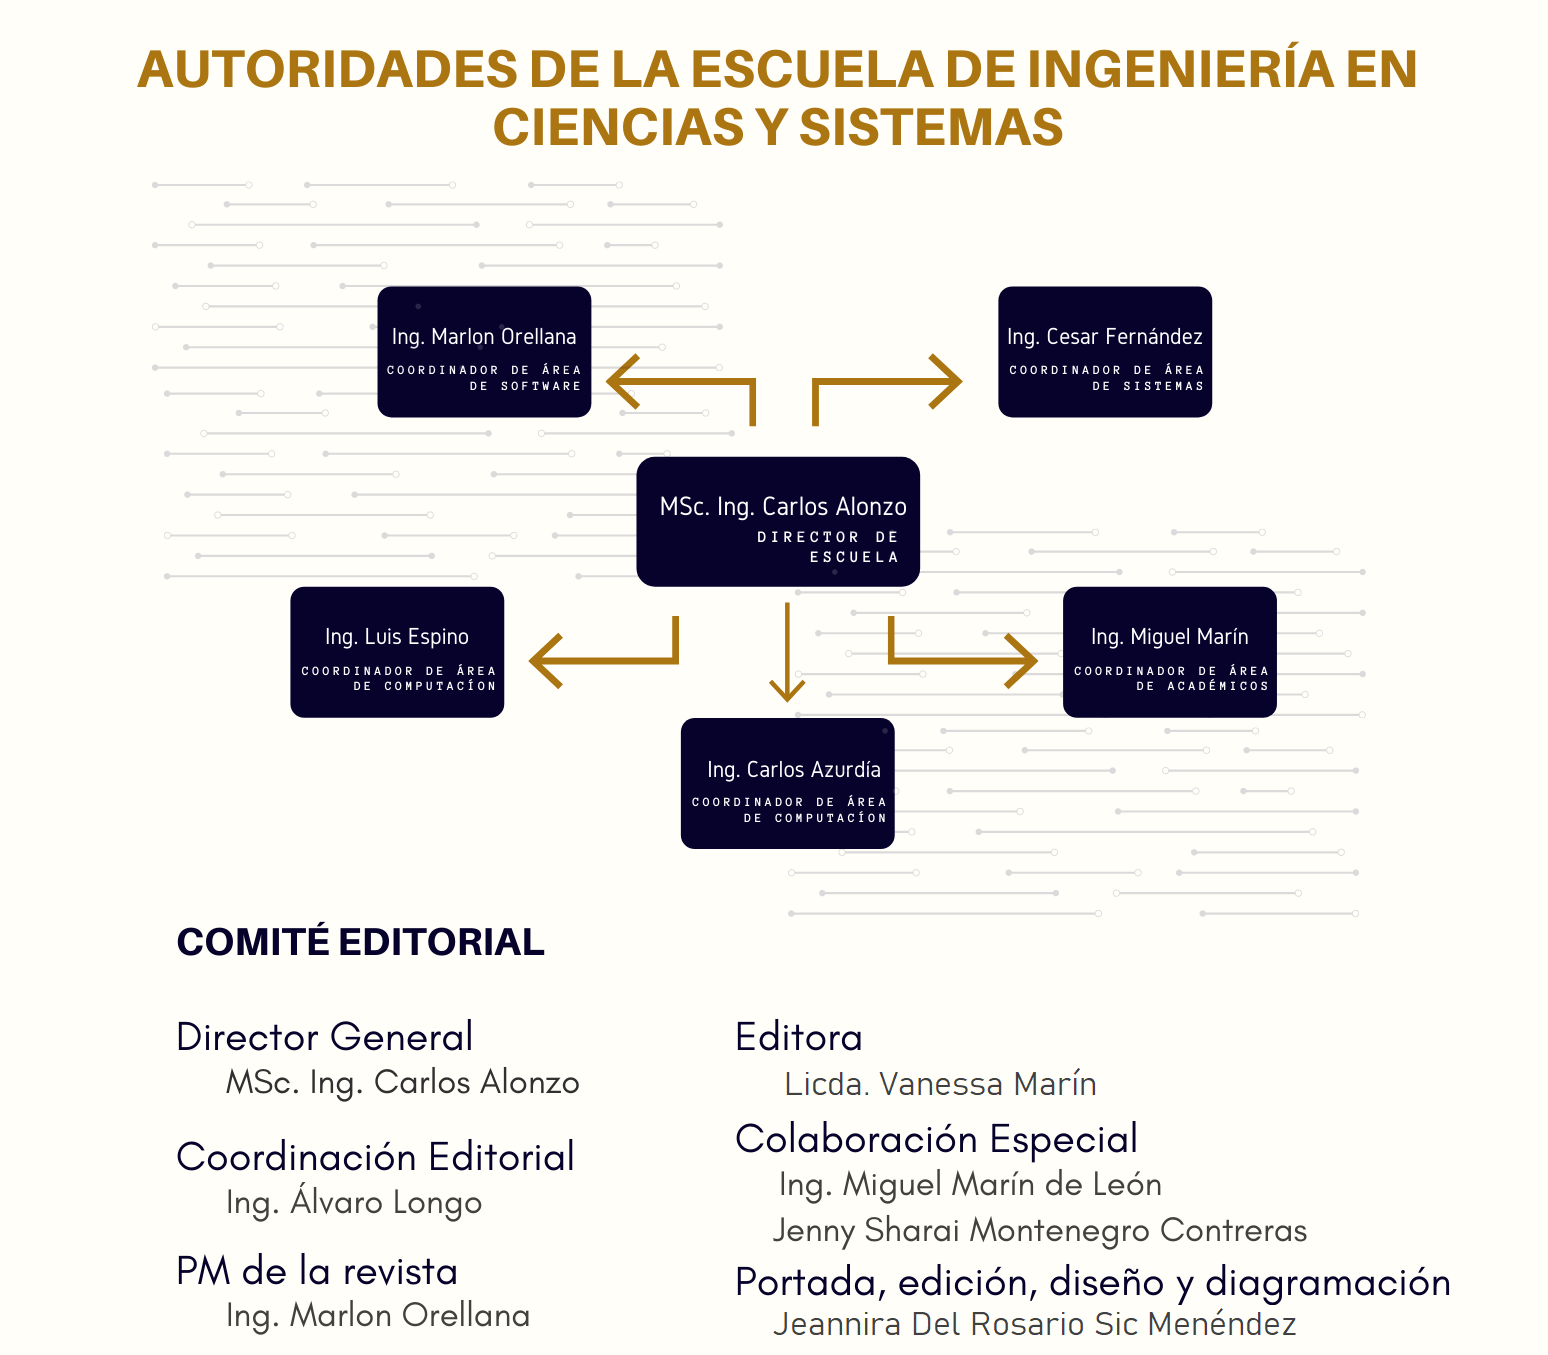
\includegraphics[width=1\linewidth]{images/organigrama} \end{center}

\hypertarget{editorial}{%
\chapter*{Editorial}\label{editorial}}
\addcontentsline{toc}{chapter}{Editorial}

\begin{center}
\includegraphics[width=1\linewidth]{images/editorial} \end{center}

\setcounter{tocdepth}{0}
\tableofcontents

\articletitlecommand

\titlespacing*{\chapter} {0pt}{-39pt}{0pt}

\hypertarget{pareja26}{%
\chapter{Inteligencia Artificial: Herramientas de finalización de código}\label{pareja26}}

\begin{center}
\includegraphics[width=1\linewidth]{images/pareja26_image1} \end{center}

\begin {multicols}{2}

En la actualidad, contamos con una gran variedad de herramientas desarrolladas en distintos lenguajes de programación, que tienen como objetivo facilitar el trabajo de los desarrolladores de software. Existen herramientas que facilitan el ciclo de vida del software, integración continua y despliegue continuo, o que permiten realizar pruebas y análisis de la calidad de un código fuente. Sin embargo, han surgido unas cuantas herramientas que desde su lanzamiento han generado debate sobre el impacto que podrían tener a futuro en la industria del desarrollo de software. Las herramientas de completado o finalización de código; tales como Github Copilot o Tabnine ¿Significa esto el fin de los desarrolladores? ¿Serán capaces de reemplazarlos? ¿Bajar la demanda competitiva en el mercado? Es necesario analizar que son realmente estas herramientas, y cuál es su verdadero propósito para dar respuesta a esta y muchas otras interrogantes. Por lo tanto, analizaremos cómo impactan estas herramientas con inteligencia artificial sobre el trabajo que realizamos como desarrolladores de software.

\hypertarget{artuxedculo}{%
\section{Artículo}\label{artuxedculo}}

La idea de reemplazar a los humanos no es para nada nueva. Hace años, desde que aparecieron los primeros sistemas automatizados, han existido personas que creen que los humanos seremos reemplazados y seremos inútiles ante el avance tecnológico. Sin embargo, muchos ignoran la realidad de los sistemas, y el verdadero beneficio que estos pueden representar al realizar tareas y procesos. Para quienes tenemos un background en la informática o desarrollo de software, este tipo de ideas realmente no debería causar ningún tipo de situación alarmante. Pero, ¿qué son las herramientas de finalización de código inteligente?

Entrando en contexto, el término ``finalización de código'' puede entenderse como un autocompletado o predicción de palabras. Este concepto no es tan nuevo, puesto que ya existen algunos editores de texto que tienen esta función integrada, donde el editor predice palabras o texto que el usuario está tratando de escribir. Esto permite acelerar las interacciones entre el usuario y el software, especialmente cuando las palabras tienen una predicción correcta. Estas funciones de autocompletado siguen algoritmos donde aprenden nuevas palabras después que el usuario las ha escrito una cantidad considerable de veces, para así hacer sugerencias. Partiendo de esta idea, ¿cuál es el ``plus'' de las herramientas de finalización de código inteligente?

\textbf{Github Copilot}

\begin{itemize}
\tightlist
\item
  ``El software se está comiendo el mundo, pero la IA se va a comer el software.'' -- Jensen Huang, Nividia CEO (2017)
\end{itemize}

Copilot a diferencia de otras IA otras existentes es que desarrolla su lógica conforme a la información a la que tiene acceso, github copilot hace uso de ``miles de millones líneas de código público existentes en repositorios, pone el conocimiento a nuestro alcance, ahorrándonos tiempo y apoyándonos en el enfoque de nuestra aplicación'', otra cosa importante es que Copilot va aprendiendo y evolucionando con el tiempo.

En ocasiones sin darnos cuenta, realizamos tareas repetitivas y Copilot es capaz de detectar esto y optimizar mejor nuestro tiempo. También a base de instrucciones puede hacer varias proyecciones de código y darnos la opción de seleccionar la que más se ajusta a nuestra instrucción.

\textbf{Tabnine}

Tabnine actualmente ofrece muchas más caracterí-
sticas de autocompletado que Copilot, pero esto se debe a que lleva mucho más tiempo en el mercado. Ambos ofrecen autocompletado de código basado en machine learning, lo que los separa es que Tabnine procesa el código línea por línea. Tabnine se encuentra en fase `producción' por lo que ofrece mejor predicción sobre Copilot y tiene mejores análisis predictivo en los diferentes lenguajes de programación.

\textbf{Diferencias entre algunas herramientas de autocompletado}

\begin {flushleft}
\noindent\begin{minipage}[c]{\columnwidth}

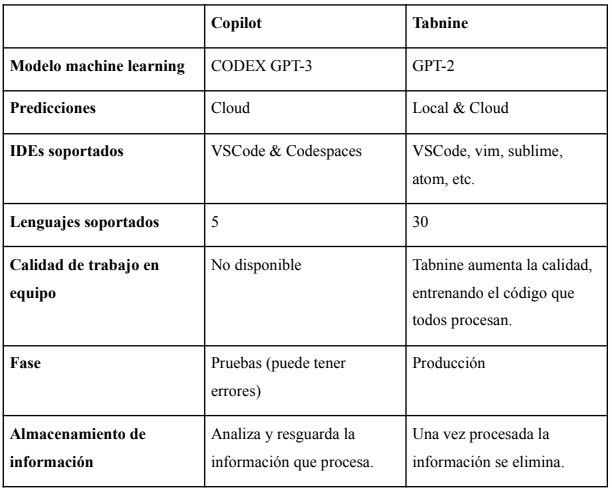
\includegraphics[width=1\linewidth]{images/pareja26_image2}
\figcaption{Tabla comparativa, Copilot de github contra Tabnine. Fuente: http://bitly.ws/pjgC}

\end{minipage}

\end {flushleft}

\hypertarget{conclusiuxf3n}{%
\section{Conclusión}\label{conclusiuxf3n}}

\begin{itemize}
\tightlist
\item
  Las aplicaciones con IA no reemplazarán a los desarrolladores, no de momento; pero hay que estar atentos a los cambios tecnológicos. Es muy complicado predecir cuándo se lanzará una herramienta capaz de tener un mejor nivel de comprensión y aprendizaje para poder ponerse a la par que un desarrollador. Pero de lo que podemos estar seguros es que estas herramientas buscan servir como asistentes y ayudantes de los desarrolladores, facilitándonos de esta forma nuestro trabajo.
\end{itemize}

\hypertarget{referencias}{%
\section{Referencias}\label{referencias}}

\begin{itemize}
\item
  {[}1{]} {[}Tabnine{]}{[}GitHub Copilot vs.~Tabnine{]}. Recuperado de: \url{http://bitly.ws/pjgC}. {[}Último acceso: marzo 2022{]}.
\item
  {[}2{]} {[}GitHub Copilot{]}{[}Your AI pair programmer{]}. Recuperado de: \url{http://bitly.ws/pjgG}. {[}Último acceso: marzo 2022{]}.
\item
  {[}3{]} {[}Pit, Catalin{]}{[}Will artificial intelligence Replace Developers{]}. Recuperado de: \url{http://bitly.ws/pjgJ}. {[}Último acceso: marzo 2022{]}.
\item
  {[}4{]} {[}Laborfox{]}{[}¿Podrá la inteligencia artificial reemplazar a un buen trabajador?{]}. Recuperado de: \url{http://bitly.ws/pjgL}. {[}Último acceso: marzo 2022{]}.
\end{itemize}

\end {multicols}
\medskip
\HRule
\medskip

\begin{center}
\includegraphics[width=1\linewidth]{images/publicidad1} \end{center}

\hypertarget{pareja27}{%
\chapter{Todo lo que necesitas saber sobre la oportunidad de la década para desarrolladores: realidad virtual}\label{pareja27}}

\begin{center}
\includegraphics[width=1\linewidth]{images/pareja27_image1} \end{center}

\begin {multicols}{2}

\hypertarget{introducciuxf3n}{%
\section{Introducción}\label{introducciuxf3n}}

Las nuevas tecnologías y tendencias en el mundo del software son el pan de cada día. Por esto, muchas veces es difícil mantener el ritmo de cuáles son los nuevos lenguajes de programación, las tecnologías, las nuevas tendencias de desarrollo. De todas las tendencias de desarrollo, aprender VR es la mejor apuesta. La realidad virtual es la tecnología que cambiará por completo el mundo del software, y es un cambio seguro, diferente a tantos otros lenguajes y tecnologías que no sabemos si van a funcionar o no en el largo plazo.

\textbf{La revolución de la realidad aumentada}

En los últimos años, muchas empresas multinacion-
ales tecnológicas han empezado a desarrollar productos relacionados con la realidad virtual. El surgimiento de esta nueva tecnología puede cambiar por completo la forma en la que trabajamos, socializamos y vivimos. Los primeros ejemplos populares de la entrada de esta industria incluyen, por ejemplo, la entrada de los Google Glass, unos anteojos de realidad aumentada que llegaron muy rápido al mercado. También tenemos el ejemplo viral del juego Pokémon Go, una manera sencilla en la que la realidad aumentada tenía contacto por primera vez con muchos usuarios.

Estos primeros ejemplos solo fueron el inicio. Hoy en día, la mayoría de empresas grandes están iniciando sus proyectos. Como ejemplo actual tenemos el Metaverso recientemente anunciado por Facebook, que tendrá un impacto social gigantesco, al tener Facebook unos 1929 millones de usuarios activos al día. Viendo esta entrada de las grandes empresas tecnológicas del mundo, ¿Cuántas nuevas oportunidades y empleos de desarrollo traerá la realidad aumentada? Según hired.com ``Esta evolución ha abierto la puerta a innumerables oportunidades para los desarrolladores de realidad virtual''.

\textbf{Un crecimiento sin competencia en la oferta de empleo}

Entre 2018 y 2019, el crecimiento de empleos disponibles para realidad aumentada creció un 1400\% (Shirin Ghaffary y Rani Molla 2020). Si lo comparamos con el desarrollo de videojuegos, que es la siguiente área por crecimiento de empleo, este nada más tuvo un 146\% de crecimiento de empleo. Eso significa que el número de empleos de realidad aumentada está creciendo 10 veces más que cualquier otra tecnología o industria de software. En la siguiente gráfica comparativa se muestra y aprecia la diferencia entre la realidad aumentada y las demás industrias de desarrollo:

\begin {flushleft}
\noindent\begin{minipage}[c]{\columnwidth}
\centering

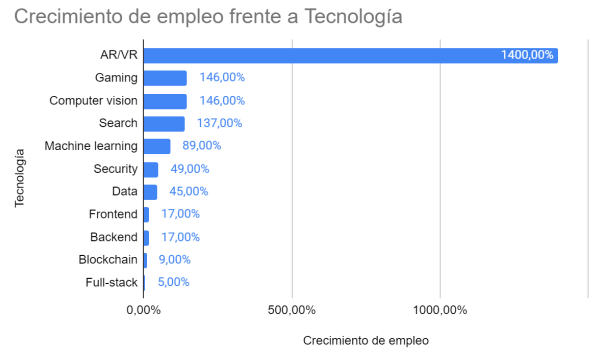
\includegraphics[width=1\linewidth]{images/pareja27_image2}
\figcaption{Crecimiento de empleo frente a tecnología. Fuente: Elaboración propia}

\end{minipage}
\end {flushleft}

\textbf{Una vista al futuro de la realidad aumentada}

El crecimiento de empleos en la realidad virtual en los últimos años ha sido impresionante. Ahora, queremos voltear al futuro para ver el número de empleos que se generarán con esta tendencia. En 2019, había 0.82 millones de empleos para realidad virtual en el mundo. Para saber cómo será el futuro, hemos acudido a Statista.com, la consultora de estadística más fiable hoy en día.

En 2030, habrá 23.36 millones de empleos de desarrollo y mantenimiento de realidad aumentada en el mundo (Statista.com 2019). Eso significa que, en solo 11 años, habrán sido creados más de 19 millones de empleos, y solo estamos hablando del inicio de esta tecnología. En la siguiente gráfica tenemos los empleos para realidad aumentada en millones entre 2019 y 2030.

\begin {flushleft}
\noindent\begin{minipage}[c]{\columnwidth}

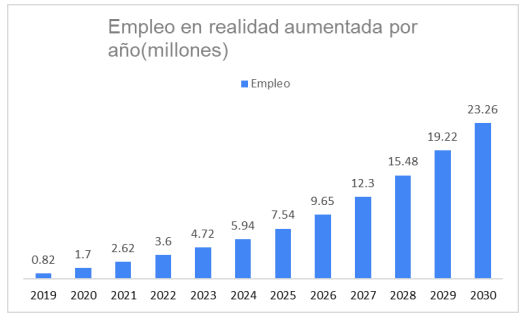
\includegraphics[width=1\linewidth]{images/pareja27_image3}
\figcaption{Empleo en realidad aumentada por año (millones). Fuente: Elaboración propia}

\end{minipage}
\end {flushleft}

\hypertarget{conclusiuxf3n-1}{%
\section{Conclusión}\label{conclusiuxf3n-1}}

\begin{itemize}
\tightlist
\item
  El surgimiento de la realidad aumentada cambiará por completo la manera en la que trabajamos, debido al gran aumento de empleos que según las estadísticas de Statista.com surgirán a lo largo de esta década. A día de hoy, el alcance de la realidad aumentada tanto en el entorno laboral como en el personal es incuestionable, pero, ¿cuáles son sus límites? es algo que sin duda tendrá respuesta con el paso del tiempo.
\end{itemize}

\hypertarget{referencias-1}{%
\section{Referencias}\label{referencias-1}}

\begin{itemize}
\item
  {[}1{]} {[}Ghaffary, Shirin y Molla, Rani{]}{[}How tech companies are trying to make augmented and virtual reality a thing, again{]}. Recuperado de: \url{http://bitly.ws/pjho}. {[}Último acceso: marzo 2022{]}.
\item
  {[}2{]} {[}Hired{]}{[}Salary range for AR/VR Engineers{]}. Recuperado de: \url{http://bitly.ws/pjhu}. {[}Último acceso: marzo 2022{]}.
\item
  {[}3{]} {[}Gajsek, Dejan{]}{[}10 In-Demand AR and VR Jobs{]}. Recuperado de: \url{http://bitly.ws/pjhx}. {[}Último acceso: marzo 2022{]}.
\item
  {[}4{]} {[}Statista 2022{]}{[}Number of jobs enhanced by augmented reality (AR) and virtual reality (VR) worldwide from 2019 to 2030{]}. Recuperado de: \url{http://bitly.ws/pjhz}. {[}Último acceso: marzo 2022{]}.
\end{itemize}

\end {multicols}
\medskip
\HRule
\medskip

\begin{center}
\includegraphics[width=1\linewidth]{images/publicidad2} \end{center}

\hypertarget{pareja51}{%
\chapter{Algoritmo salva vidas}\label{pareja51}}

\begin{center}
\includegraphics[width=1\linewidth]{images/pareja51_image1} \end{center}

\begin {multicols}{2}

\hypertarget{introducciuxf3n-1}{%
\section{Introducción}\label{introducciuxf3n-1}}

La inteligencia artificial es uno de los campos de la informática más relevantes hoy en día, no es un secreto que varios problemas cotidianos que se nos hacían complejos hasta hace unos años, se han podido resolver por medio de algoritmos diseñados para aprender un conjunto de patrones y que maximicen la posibilidad de éxito de un objetivo. Esto se ha aprovechado muy bien en diferentes ámbitos de todas las industrias, la medicina no ha sido la excepción.

El despliegue de la inteligencia artificial persigue varios objetivos como la mejora de las condiciones de vida de las poblaciones, la personalización del precio de la atención médica, el estímulo de la innovación y la productividad. Estas tecnologías pueden llegar a modificar los límites entre el hombre y la máquina.

Existen muchos mitos sobre sí la inteligencia artificial es ``sólo una moda'' y que, si esta no ha avanzado lo suficiente en los últimos años, pero la verdad es que en el campo de la medicina ha ayudado a varios expertos a detectar anomalías en sus pacientes antes de tiempo y poder tratar la enfermedad con antelación para mitigar la enfermedad.

\textbf{Inteligencia artificial y salud}

La inteligencia parece ser la capacidad que poseemos para resolver problemas o adaptarnos a un entorno, tanto mental como cognitivamente. Los científicos tienden a reducir la inteligencia al cerebro, porque en los animales, la inteligencia se realiza a través de sistemas neuronales. Ahora con la inteligencia artificial, que puede definirse como ``Disciplina científica que se ocupa de crear programas informáticos que ejecutan operaciones comparables a las que realiza la mente humana, como el aprendizaje o el razonamiento lógico'' vamos a reducir la inteligencia a la capacidad de aprender y responder lógicamente a las expectativas, en función de las capacidades del cerebro.

La inteligencia artificial ``débil'' es la IA que podemos crear en este momento, es una inteligencia artificial que se enfoca en una tarea específica: misión dada, respuesta a la misión dada. No es capaz de sentir emociones o sentimientos y no es sensible. Hoy en día, todas las inteligencias artificiales se consideran débiles. El caso más maduro de IA en la actualidad es el utilizado para reconocimiento de imágenes de melanoma.

\textbf{Medicina predictiva}

El concepto de medicina predictiva fue utilizado por primera vez en 1972 por el profesor de medicina experimental Jean Dausset, Premio Nobel de Medicina. Primero, ¿qué es la medicina predictiva? Tomando la definición de la web de la asociación para el progreso de la biología médica, ``la medicina predictiva se basa en la detección en un individuo de predisposiciones biológicas a tal o cual enfermedad, con el fin de retrasar, atenuar o incluso prevenir su aparición''. Así, en definitiva, la medicina predictiva pretende anticipar los riesgos de determinadas enfermedades mediante el análisis de los genes, o incluso tratarlas y evitarlas.

\textbf{IA en medicina}

A principios de los años 70 se creó un sistema experto (sistema que emula el razonamiento humano) llamado Mycin utilizado para identificar bacterias que causan infecciones graves y recomendar antibióticos, este tenía solo un 65\% de diagnósticos correctos en 1979 y ya había logrado vencer a los cinco expertos en enfermedades infecciosas de Stanford University Medical Center, juzgados en las mismas condiciones, con desempeños individuales que van del 42,5\% al 62,5\% de diagnósticos correctos.

Durante la década de los 70 se desarrollaron varios sistemas expertos que fueron pioneros en el uso de la inteligencia artificial no solo para el área médica sino también para otras áreas como la geología con Prospector y la computación con Age, OPS5, Rosie o R1.

\begin {flushleft}
\noindent\begin{minipage}[c]{\columnwidth}
\centering

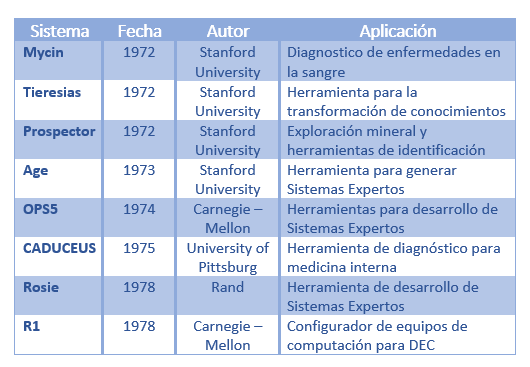
\includegraphics[width=1\linewidth]{images/pareja51_image2}
\figcaption{Sistemas expertos pioneros. Fuente: Elaboración propia}

\end{minipage}
\end {flushleft}

En abril del 2020 el Instituto sobre Alcoholismo y Farmacodependencia (IAFA), el Ministerio de Salud de Costa Rica y la Caja Costarricense del Seguro Social (CCSS) lanzó un asistente virtual a través de Facebook que busca apoyar a los ciudadanos que quieren dejar de fumar o vapear, el rendimiento del bot de IAFA en las pruebas es de 97.57\% de verdaderos positivos y 99.15\% de verdaderos negativos, que en comparación con Mycin muestra tener un mejor rendimiento.

Otro ejemplo de aplicación de inteligencia artificial en la medicina es la reducción de la infectividad de la última crisis del ébola. Se utilizó un programa con inteligencia artificial para evaluar los diferentes medicamentos que existían para la cura del ébola, y se encontró que existían dos medicamentos que podrían reducir el porcentaje de infección de esta enfermedad. Lo más sorprendente fue que este proceso sólo duró un día, mientras que este tipo de análisis suele durar varios meses o incluso años. Este proceso sin lugar a dudas salvó a miles de personas que gracias al software con inteligencia artificial pudieron tener mucho más rápido este medicamento.

\hypertarget{conclusiones}{%
\section{Conclusiones}\label{conclusiones}}

\begin{itemize}
\item
  La inteligencia artificial en la medicina ya es una realidad, ya que está siendo aplicada en diferentes campos de la medicina. Los softwares utilizados para los análisis y las pruebas han servido como un medio de optimización de procesos, ya que la capacidad de procesamiento de una máquina es mayor al de un ser humano, debido a que la máquina se está enfocando solamente en la realización de una tarea específica y gracias a los nuevos algoritmos de redes neuronales la máquina puede seguir aprendiendo y mejorando la probabilidad de éxito de un resultado. Además, ha reducido la necesidad de experimentar con animales, lo cual está muy mal visto por parte de la sociedad.
\item
  La IA podría ser un activo importante para la medicina sin reemplazar todos los aspectos ``humanos''. Utilizar la IA como herramienta adicional para un médico humano sería positivo, pero no para sustituirlos definitivamente. Además, como herramienta, el profesional de la salud no debe confiar completamente en la IA porque, por definición, es una máquina y por lo tanto no puede ver lo que los humanos pueden ver, especialmente cuando se trata de realidades y sentimientos sociales. Siendo también cierto lo contrario en la medida en que el cerebro humano es limitado, parece necesario encontrar el justo equilibrio entre ambos para poder beneficiarse del máximo de los beneficios y del mínimo de los peligros.
\end{itemize}

\hypertarget{referencias-2}{%
\section{Referencias}\label{referencias-2}}

\begin{itemize}
\item
  {[}1{]} {[}RAE, Diccionario de la lengua española{]}{[}inteli-
  gencia{]}. Recuperado de: \url{http://bitly.ws/poaF}. {[}Último acceso: febrero 2022{]}.
\item
  {[}2{]} {[}AImPbm{]}{[}APBM: Medicina Predictiva{]}. Recuperado de: \url{http://bitly.ws/poaG}. {[}Último acceso: febrero 2022{]}.
\item
  {[}3{]} {[}Organización Mundial de la Salud{]}{[}OMS, Informe sobre inteligencia artificial{]}. Recuperado de: \url{http://bitly.ws/poaH}. {[}Último acceso: febrero 2022{]}.
\item
  {[}4{]} {[}Marqués, F.L.{]}{[}Aplicaciones de la inteligencia artificial en Medicina{]}. Recuperado de: \url{http://bitly.ws/poaK}. {[}Último acceso: febrero 2022{]}.
\end{itemize}

\end {multicols}
\medskip
\HRule
\medskip

\hypertarget{miguelsic}{%
\chapter{Como los algoritmos influencian el comportamiento humano}\label{miguelsic}}

\begin{center}
\includegraphics[width=1\linewidth]{images/mSic_image1} \end{center}

\begin {multicols}{2}

Las famosas ``ofertas'' que hemos visto desde hace muchos años, cuando salimos de compras, en grandes anuncios publicitarios, en los medios escritos, televisivos o por radio y ahora los famosos ``Ads'' (abreviatura de la palabra inglesa ``advertising'', en español ``anuncio'') que las redes sociales y programas de internet que hoy en día nos invaden conocida como ``publicidad invasiva'' y la última moda sobre la creación de canales en redes sociales llamados ``influncers'' personas que expresan opinión sobre un tema concreto y ejercen una gran influencia sobre muchos seguidores.

Esta necesidad de llevar un mensaje en su mayoría de los casos, para comercializar algún bien o servicio, para incrementar ventas, captar o retener clientes, ofrecer experiencias personalizadas o sencillamente para dar a conocer mensajes de algo a alguien, toda esta necesidad del ser humano se ha fusionado con las nuevas tecnologías de la información por medio el uso de ``algoritmos'' cada vez más inteligentes y sofisticados que tratan de imitar el pensamiento del ser humano.

Algunos ejemplos donde podemos encontrar algoritmos inteligentes son los sistemas que usan Spotify, Disney+, YouTube, NETFLIX, Facebook, Instagram, Google y Amazon; ¿has recibido alguna recomendación? para escuchar una playlist (lista de canciones), ver una película o vídeo, hacerte amigo en la red o comprar por internet; hoy trataré de explicar un poco como funcionan estos algoritmos que nos impulsan a tomar decisiones y pueden alterar nuestro comportamiento.

Existen tres tipos métodos: 1. sistema de filtrado colaborativo, 2. sistema de recomendaciones por contenido y 3. sistemas híbridos; el método inicia creando un algoritmo para determinar la similitud entre dos elementos, personas o usuarios, para ello se usan métodos como el índice de Jaccard, similitud coseno, distancia Euclidiana, y correlación de Pearson.

Los algoritmos para crear los sistemas de inteli-
gencia utilizan una matriz de utilidad que refleja la relación entre los elementos, productos y usuarios, que son los conjuntos principales de un sistema de recomendación.

Por otro lado, el método del sistema de filtrado conocidos como basado en memoria (usuario a usuario) o (producto a producto), la recomendación es más personalizado ya que las interacciones están basadas en usuarios similares al usuario de interés, sin embargo los productos recomendados suelen ser más diversos; si hablamos del método producto a producto la recomendación es más robusta, porque hay menor varianza por la cantidad de interacciones de usuarios, sin embargo puede haber sesgo por las interacciones que provienen de todo tipo de usuario.

El sistema de filtrado colaborativo basado en modelos, se basan en información de las interacciones entre el usuario y el elemento, este método hace menos complejo y denso el manejo de las matrices, los modelos usados habitualmente son el modelo de regresión, árboles de decisión, k-vecinos más cercanos y máquinas de vectores de soporte; este método combina una representación de interacciones usuario a producto, lo que permite generar recomendaciones a usuarios sin historial de interacciones, siendo siempre nuestro objetivo predecir datos muy cercanos a los valores verdaderos (conocido como BIAS).

Ahora hablaremos sobre los algoritmos para crear sistemas de recomendación por contenido, en el que perfilamos al usuario (región, edad, género, gustos, etc.) y el producto (si fuera películas serias algo como director, género, actores, año, etc.); se define el modelo centrado en los productos, el usuario o combinado; y se procede a entrenar el modelo lo que significa que tomamos una muestras de datos, según los resultados de las pruebas y entrenamientos se determina cuando es el error entre lo pronosticado y lo real, entonces usamos el ultimo conjunto de datos de validación para realizar el pronóstico.

Todo se escucha muy bien y puede que sea de mucha utilidad, sin embargo existe un debate ético sobre los sistemas de recomendaciones basados en algoritmos; Eli Parieser define el término ``filtro burbuja'' al estado de aislamiento intelectual que está influenciando el comportamiento humano, usando algoritmos inteligentes para personalizar el resultado de las búsquedas, es decir la misma búsqueda puede producir resultados distintos, esto tomando la información personal del usuario, ubicación o enlaces en los que hizo clic en el pasado; estos son aislados en sus burbujas ideológicas y culturales.

Algunos ejemplos que usualmente encontramos de filtros burbuja son: Google, filtra búsquedas de acuerdo con las otras consultas de usuarios, así como links que siguieron y muchas otras variables como la dirección IP, la marca del equipo, su ubicación, lo más relevante cuando la persona hace clic en el primer enlace.

Facebook ha explotado grandemente la interacción entre sus millones de usuarios, personalizando el contenido para proporcionar recomendaciones y sugerencias según el uso por medio de los clics, páginas visitadas, búsquedas realizadas y ahora usa motores de inteligencia artificial por medio de Deep Learning (algoritmos para reconocimiento de imágenes), es decir conocer tus gustos de vestir, lugares que has visitado, personas con las que socializas y con toda esta gama de información personaliza tu entorno.

Otro aspecto negativo de las recomendaciones y sesgos de información dentro del debate ético son las Fake News (noticias falsas) y radicalización; podemos citar la reciente pandemia de covid-19 sobre la reproducción de muchas noticias falsas, que la Organización Mundial de la Salud acuñó como ``infodemia'' a la sobre abundancia y multiplicación de noticias falsas en relación al brote epidémico.

He tratado de plantear por medio de estas nuevas modas tecnológicas que, si bien es cierto son activadores de más oportunidades en la economía mundial, también existen efectos negativos que debemos cuidar para tener una libertad intelectual en nuestras decisiones para un comportamiento equilibrado para nuestro bienestar y el de la sociedad.

\hypertarget{referencias-3}{%
\section*{Referencias}\label{referencias-3}}
\addcontentsline{toc}{section}{Referencias}

\begin{itemize}
\item
  {[}1{]} {[}Wikipedia, the free encyclopedia{]}{[}Recomme-
  nder system{]}. Recuperado de: \url{http://bitly.ws/pHQp}. {[}Último acceso: febrero 2022{]}.
\item
  {[}2{]} {[}Wikipedia, the free encyclopedia{]}{[}Filtro burbuja{]}. Recuperado de: \url{http://bitly.ws/pHQu}. {[}Último acceso: febrero 2022{]}.
\item
  {[}3{]} {[}JAYWRKR Tech{]}{[}Guía para construir un sistema de recomendación (Parte 1){]}. Recuperado de: \url{http://bitly.ws/pHQx}. {[}Último acceso: febrero 2022{]}.
\item
  {[}4{]} {[}Adamczyk, Jakub{]}{[}k nearest neighbors computational complexity{]}. Recuperado de: \url{http://bitly.ws/pHQI}. {[}Último acceso: febrero 2022{]}.
\item
  {[}5{]} {[}Wikipedia, the free encyclopedia{]}{[}Fake news{]}. Recuperado de: \url{http://bitly.ws/pHQL}. {[}Último acceso: febrero 2022{]}.
\item
  {[}6{]} {[}Wikipedia, the free encyclopedia{]}{[}Infodemia{]}. Recuperado de: \url{http://bitly.ws/pHQW}. {[}Último acceso: febrero 2022{]}.
\end{itemize}

\end {multicols}
\medskip
\HRule
\medskip

\begin{center}
\includegraphics[width=1\linewidth]{images/publicidad6} \end{center}

\hypertarget{kevinlajpop}{%
\chapter{Voto electrónico con ``blockchain'': la unión entre la tecnología y la sociedad}\label{kevinlajpop}}

\begin{center}
\includegraphics[width=1\linewidth]{images/kLajpop_image1} \end{center}

\begin {multicols}{2}

\hypertarget{resumen}{%
\section{Resumen}\label{resumen}}

La sociedad ha ido evolucionando en función del crecimiento de la tecnología, por lo que, el complejo comportamiento social se ha visto influenciado por la tecnología, así mismo se ha visto complementado por la misma. Esto no excluye un proceso electoral con la inmersión del voto electrónico, pero la creación de un voto de esta índole no es solo crear un sistema que lleve el conteo de los votos o que permita emitir un sufragio, sino debe de respetar los fundamentos del voto, entre los cuales se puede mencionar que es único por persona, privado y secreto.

Ante todo, este tipo de requerimientos, no todas las arquitecturas de software cumplen con las características tan exigentes del voto electrónico, y una de las tecnologías que llegan a cumplir estos requerimientos es el ``blockchain'', dicha tecnología sus fundamentos yacen en la privacidad, seguridad, poder distribuido, entre otras características.

\hypertarget{palabras-clave}{%
\section{Palabras clave}\label{palabras-clave}}

``Blockchain'', criptografía, democracia, transparen-
cia, consenso

\hypertarget{abstract}{%
\section{Abstract}\label{abstract}}

Society has evolved based on the growth of technology, so that complex social behavior has been influenced by technology, and has also been complemented by it. This does not exclude an electoral process with the immersion of electronic voting, but the creation of a vote of this nature is not only to create a system that keeps the votes counting or that allows voting to be cast, but must respect the fundamentals of the vote, among which it can be mentioned that it is unique per person, private and secret.

Given all these types of requirements, not all software architectures meet the demanding characteristics of electronic voting, and one of the technologies that meet these requirements is the ``blockchain'', said technology, its foundations lie in privacy, security, power. distributed, among other features.

\hypertarget{keywords}{%
\section{Keywords}\label{keywords}}

``Blockchain'', cryptography, democracy, transparen-
cy, consensus

\hypertarget{introducciuxf3n-2}{%
\section{Introducción}\label{introducciuxf3n-2}}

El mundo está atravesando una cuarta revolución industrial, una revolución que no hace alusión a la tecnología disruptiva como lo ha sido en anteriores revoluciones (Escudero, 2018) sino a lo transversal que pueden llegar a ser las disciplinas, como, por ejemplo, las ciencias de la computación aplicadas a la medicina o la robótica aplicada a la manufactura. Esto ha dado nacimiento a nuevas disciplinas, como lo ha sido la hiperconectividad, internet de las cosas, el auge de la ciencia de datos o nuevas infraestructuras como lo es el ``blockchain'' (González-Páramo, 2018).

Tal y como menciona Aretio (2019), la forma de vivir de la sociedad se verá en la necesidad de ser modificada a raíz de los avances de las Tecnologías de la Información y Comunicación, en adelante TIC, no únicamente impacta en la industria como tal, sino también en la forma de vivir de las distintas sociedades dado que la cuarta revolución industrial está creando ecosistemas digitales en los cuales los individuos estén conectados (Escudero, 2018).

Y al momento de hablar de sociedad y tecnología, no se puede hacer a un lado a la administración pública ni al estado porque el avance de las TIC también impacta al sector público, dado que, la modernización del estado es una oportunidad de desarrollo y crecimiento económico, social, cultural entre otras áreas (Xavier, 2016); y a todo esto se le denomina gobierno electrónico, que no es más que el uso de las TIC como un pilar en la administración pública, como lo es en la prestación de servicios públicos, transparencia, auditoría social o la optimización de procesos. Cuando se toca el tema de optimización de procesos, se puede mencionar un proceso tan complejo como lo es el sistema electoral, el cual es profundo porque tiene muchas aristas en lo social, tecnológico, innovación e incluso en la política.

\hypertarget{planteamiento}{%
\section*{Planteamiento}\label{planteamiento}}
\addcontentsline{toc}{section}{Planteamiento}

\textbf{Voto y sociedad}

Según Ocaña (1999), un sistema electoral es el proceso en el cual los ciudadanos o miembros de una sociedad manifiestan una preferencia por otro grupo de personas, para que asuman la autoridad y administración para la cual se está realizando dicho proceso. En el sistema electoral existen varios actores que regulan el buen funcionamiento del mismo y esto con base a un conjunto de reglas que norman dicho sistema.

De igual manera, es necesario saber que en un movimiento electoral existen tres perspectivas mínimas que hay que tener en cuenta, siendo la primera; los puestos que están en disputa y a elección, en esta perspectiva se determina quién gana o quién pierde, que a la larga es el objetivo del proceso electoral, como segunda perspectiva está la participación de la sociedad; siendo esto, incluso, un derecho con el que cuentan las personas en algunas sociedades y la última perspectiva es la decisión de cada persona que emite su sufragio, es la orientación o preferencia electoral de la persona (Vallés, 1990).

Se puede asegurar que el voto es un comportamie-
nto individual y social, dado que nace de un individuo con el pensamiento y orientación electoral con el que se identifica, pero el sistema electoral lo constituye una sociedad con sus diferentes actores, porque existen personas que determinan las reglas, otros que se postulan a elección y por último quiénes eligen a las personas que se han postulado con base a las reglas, que la misma sociedad, por medio de personas idóneas las han determinado.

Un proceso electoral tiene sus fundamentos en la legitimidad y credibilidad, esto provoca en la población votante, una madurez y también interés por dicho proceso, no solo en participación, sino en la postulación, así como en la ejecución de dicho mandato, para el cual se está llevando a cabo el escrutinio. Todo esto desemboca en una sociedad apática y que rechaza la opacidad de los procesos electorales, por lo que se puede concluir que, para un proceso electoral, es importante la transparencia y rendición de cuentas (Vázquez, 2020).

El voto es la unidad mínima de un sistema electoral, dado que es único por persona y es por lo cual existe la disputa electoral, pero la realización de comicios es mucho más compleja, porque existe un sinfín de variables que hay que tomar en cuenta en este sentido, por mencionar algunos, insumos físicos, personal masivo o una estrategia y logística que prevea todos los escenarios posibles. Al momento de hablar de una actividad social de esta envergadura, hay que ver los posibles fallos que puede tener este proceso, como es el manejo y manipulación de boletas, tiempo en lo que se realiza el escrutinio, entre otros (Montes, 2016); y cuando existe una complicación o un alto riesgo en la elaboración de los comicios se pierde los fundamentos necesarios para llevar a cabo un proceso electoral sano.

\textbf{El voto electrónico}

En la actualidad la tendencia es automatizar vía las TIC las acciones y procesos sociales, no dejando esta automatización solo para la iniciativa privada, sino también para la administración pública y eso puede incluir un proceso electoral, pero este tipo de implementaciones está lejos de ser una realidad en países de Latinoamérica (Montes, 2016), esto a raíz de que no es una característica esencial dentro del desarrollo de la sociedad latinoamericana.

Pero a todo esto, ¿qué se entiende como voto electrónico?, según Montes (2016) el voto electrónico es aquel proceso electoral en el cual la emisión del voto y el escrutinio de los mismos están bajo el uso de computadoras, esto deja claro, para que se cuente con un sistema de votación electrónica no basta solo con la digitación de los resultados o con tener gráficas y datos tabulados en línea, sino en todo el proceso se debe de contar con un dispositivo electrónico que procese el voto, desde su emisión hasta su escrutinio.

En la actualidad, el tener un voto electrónico va más allá de tener un sistema de información y esto es debido a la naturaleza de este, porque un sistema electoral es muy complejo y encontrar la armonía entre un sistema social y un sistema computacional es el verdadero reto, pero con el avanzar del tiempo y la cuarta revolución industrial se hace cada vez más necesario el contar con el voto electrónico.

\hypertarget{desarrollo}{%
\section{Desarrollo}\label{desarrollo}}

\textbf{Desmintiendo el voto electrónico}

Existen varias aseveraciones que no son ciertas y que giran en torno al voto electrónico tal y como dicta Vilamala (2014), las cuales, en varias ocasiones son obstáculos que tienen las sociedades para poder llevar a cabo un proceso electoral electrónico, siendo estas las siguientes:

\begin{enumerate}
\def\labelenumi{\arabic{enumi}.}
\item
  El voto electrónico solo es en internet, es necesario tener en cuenta que, para la realización de un proceso electoral digital, no es estrictame-
  nte vía internet sino se pueden emplear otras técnicas tecnológicas que pueden apoyar en la comunicación del sufragio.
\item
  El voto electrónico es solamente para entornos no controlados o no convencionales, es importante definir que un sistema electoral, por lo regular, es un entorno controlado y también auditado, porque tiene reglas procedurales y de igual manera jurídicas, por lo que se debe tener en cuenta que, el hecho que exista una votación electrónica no es significado de incerteza jurídica o desorden, y viceversa.
\item
  El voto electrónico es solo para elecciones políticas en una sociedad macro, sino el voto electrónico es transversal para elecciones de cualquier índole, por ejemplo, un gobierno universitario, elección de comités, juntas directivas u otro tipo de proceso electoral democrático que lleva a cabo la sociedad, por lo tanto, el sufragio electrónico va orientado a la necesidad de elección que tiene la sociedad, no a la política electoral o partidaria nacional.
\item
  El voto electrónico solamente es para países con un poder adquisitivo mayor, tal y como menciona Vilamala (2014) existen varios países que no cumplen con este enunciado, dado que no es cuestión monetaria, sino es cuestión cultural la adaptación del voto electrónico, porque no hay ninguna tendencia a que, países con más poder adquisitivo, tengan un sistema electoral electrónico.
\end{enumerate}

\textbf{Retos del voto electrónico}

El voto electrónico presenta dos tipos de retos o dificultades a vencer, y son los retos de tipo técnicos y teóricos (Montes, 2016):

\begin{itemize}
\tightlist
\item
  Reto técnico: al momento de que el voto sea electrónico o digital, tiende a tener los mismos problemas que puede presentar un sistema de información normal, siendo estos los típicos problemas de seguridad, alta disponibilidad, ataques internos o externos que son, a su vez, problemas del día a día de un sistema (Montes, 2016), pero al momento de hablar del voto electrónico, dichos problema no deben de pasar, el margen de error debe de tender a cero.
\end{itemize}

Otro reto que se puede detectar es la privacidad y seguridad de la información, el sistema de votación electrónica debe de asegurar que los votos no podrán ser alterados bajo ningún término, tampoco que se pueda identificar la decisión de una persona al momento de emitir su sufragio, por lo que el papel que juega la criptografía en un sistema electoral digital es clave, así como el reto de implementar un sistema criptográfico infalible es complejo (Jaramillo, 2015).

\begin{itemize}
\item
  Reto teórico: un sistema electoral debe tener varios requisitos tal y como los tiene un sistema electoral normal, entre estos requisitos, Jaramillo (2015) plantea los siguientes requisitos vitales:

  \begin{itemize}
  \item
    Elegibilidad, es cuando una persona forma parte del padrón electoral, no todas las personas de una sociedad son aptas para ejercer el voto;
  \item
    Unicidad es uno de los retos más grandes del sistema electoral, dado que es la propiedad que indica que, ninguna persona debe de poder votar más de una vez por cada justa electoral;
  \item
    Precisión, en una justa electoral los datos deben de ser precisos, deben de reflejar tal cual pasó la dicha contienda, no debe existir falta de votos o sobrante de los mismos;
  \item
    Verificable y transparente, los votos deben poderse verificar, es decir, que los votos emitidos sean los que se cuentan al final del proceso electoral, esto es a la larga un proceso de transparencia que también es necesario para el sistema electoral digital;
  \item
    Privacidad y seguridad, el sistema electoral debe de ser privado y seguro, partiendo de un voto no se puede identificar al emisor de dicho voto, se le debe de guardar la privacidad del votante, lo único que se debe de poder saber es el voto como tal, pero jamás quién emitió ese voto.
  \end{itemize}
\end{itemize}

Así mismo también se debe de tener en cuenta que el sistema electoral tiene que ser seguro, en ningún momento se debe de ponerse en contienda la integridad de la persona, seguridad en cualquier ámbito, ya sea seguridad física o seguridad informática.

No es tan sencillo implementar un sistema electoral electrónico, en el cual se tenga la certeza que los retos técnicos y teóricos se cumplan a exactitud, dado que, con la creación de un sistema de información convencional no se puede lograr esa privacidad tan ansiada que se busca, por mencionar un reto. Son pocas las tecnologías que pueden hacer alusión a la privacidad, seguridad, transparencia, entre otras características; lo que, a la larga, todo apunta a la tecnología que soporta al bitcoin: el ``blockchain''.

\textbf{``Blockchain''}

El Blockchain o cadena de bloques es una tecnología del tipo de estructura de datos, que funciona como un libro mayor en el cual se registran transacciones que se almacenan dentro de bloques, dicho libro o cadena de bloques se almacena en todos los miembros de la red, es decir, todos los miembros de la red guardan una copia del registro de las transacciones (Bashir, 2017), así teniendo su poder, no en un modelo monolítico sino en el poder distribuido, de igual manera, no hay una sola fuente de verdad absoluta de los datos, sino que todos a su vez tienen la fuente verdadera de datos.

\textbf{Los principio del ``Blockchain''}

El ``blockchain'', como toda tecnología, tiene principios que marcan la diferencia y el rumbo a seguir al momento de implementar esta tecnología, según Tapscott (2017) una aplicación ``blockchain'' debe de contar con principios mínimos, siendo los siguientes:

\begin{enumerate}
\def\labelenumi{\arabic{enumi}.}
\item
  Integridad, al momento de no contar con un componente aislado que contenga la verdad absoluta, hace que la integridad esté a lo largo de la cadena, a razón de que al momento que todos tengan una copia del libro de transacciones, todos tienen la verdad absoluta y el elemento de la cadena que tenga un diferencial en su libro de transacciones, se identificará como un intento de alteración, pero la mayoría dará la integridad de los datos y las transacciones.
\item
  Poder distribuido, el hecho de ser una tecnología descentralizada no existe el poder centralizado, sino el poder radica en lo descentralizado en lo que se encuentra la red ``blockchain''.
\item
  Seguridad, el hecho que las transacciones o datos estén resguardados en todos los nodos de la red, no dicta que los nodos tengan acceso a dichas transacciones, sino las transacciones y datos de la cadena están resguardados con altos mecanismos criptográficos ya sean simetricos o asimetricos, dependiendo del caso, así será el algoritmo criptográfico que se utilizará.
\item
  Privacidad, los datos de una transacción únicamente pueden ser accedidos por el dueño de la transacción con una contraseña o clave con la que fue cifrada, dicha información o transacción no puede ser accedida por ninguna otra persona, a menos que tenga la contraseña o clave.
\end{enumerate}

El ``blockchain'' puede tener más principios o características, dependiendo del autor o investigador, pero las anteriores descritas son los pilares del ``blockchain'', haciendo de esta, una tecnología que está orientada a la privacidad, seguridad y transparencia de transacciones. En la figura 1 se puede observar cómo interactúan los miembros de la red de ``blockchain'' y el registro del libro contable los cuales todos los nodos de la red tienen acceso.

\begin {flushleft}
\noindent\begin{minipage}[c]{\columnwidth}
\centering

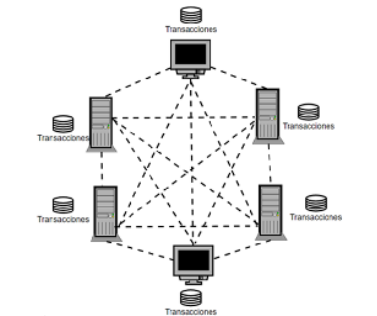
\includegraphics[width=1\linewidth]{images/kLajpop_image2}
\figcaption{Red de "Blockchain". Fuente: Elaboración propia}

\end{minipage}
\end {flushleft}

\textbf{El concenso}

A toda esta teoría, ¿cómo es que el ``blockchain'' acepta las transacciones?, ¿cómo se ponen los nodos de acuerdo sobre una transacción nueva?, pues esa es la última pieza del ``blockchain'', a este proceso de aceptación de transacciones y puesta de acuerdo de todos los participantes se le denomina consenso, el consenso se realiza de manera digital y automático, es un proceso de votación en la cual todos los nodos que son parte de la red, tienen representación y según Gupta (2017), el consenso tiene las siguientes características clave:

\begin{itemize}
\item
  Prueba de participación: es la forma en la que se valida las transacciones, por lo regular es contar con un cierto porcentaje del valor total de los miembros de la red, es decir, la mayoría debe de estar de acuerdo de cualquier inserción en la cadena de transacciones, al momento que no exista un acuerdo no se acepta la transacción y será debido a la falta de mayoría.
\item
  Firma múltiple: al momento de que todos participan a su vez, firman la transacción por lo que estará validado electrónicamente dicha transacción.
\item
  Tolerancia a falla bizantina: una red ``blockchain'' en su concepción, tiene que cumplir con tener un plan de acción ante una falla bizantina, dicha falla bizantina puede ser falla de red, falla de validación, falla de tiempo de espera, entre otros.
\end{itemize}

Al final, el consenso es el mecanismo digital con el cual una transacción se hará válida, una transacción puede ser un voto electrónico, por lo tanto, para que un voto electrónico sea válido todos los miembros o nodos de la red ``blockchain'' deben de aceptar la transacción con la mayoría de los nodos a favor de la nueva transacción o voto.

\textbf{El ``Blockchain'' y el voto electrónico}

La tecnología ``blockchain'' es un mecanismo digital en el cual prevalecen inquebrantables todas las transacciones, haciendo imposible que exista una modificación o alteración de esta, con esto logrando una transparencia digital máxima y por medio de los algoritmos criptográficos que conlleva esta tecnología se asegura la privacidad de todas las transacciones.

Teóricamente, pareciera que el sistema electoral calca perfectamente con la funcionalidad del ``block-
chain'', pero no es fácil converger un sistema social tan complejo como el de un proceso electoral, aunque ``blockchain'' es la tecnología adecuada, es necesario tener en cuenta los retos anteriormente descritos, porque son los retos que debe de superar esta tecnología.

\textbf{Perspectiva del futuro}

En un momento dado las sociedades verán la necesidad de contar con un sistema electoral electrónico o un híbrido, para ello se tendrá que tener en cuenta la tecnología ``blockchain'' para la implementación del proceso electoral, pero también es de conocimiento que ``blockchain'' no será la solución para los problemas sociales, culturales o electorales, la implementación de un sistema con esta tecnología traerá consigo solución de problemas, ventajas o ganancias sobre el modelo tradicional, pero de igual manera traerá nuevos retos, problemas o situaciones que no habían sido exploradas en con modelo tradicional.

La necesidad del voto electrónico ha ido creciendo conforme al pasar el tiempo (Vilamala, 2012), llegando a ser una necesidad de la sociedad, pero cada segmento poblacional es diferente, por lo que es necesario un estudio exhaustivo de dicha evolución del sistema electoral, en el cual se incluya todos los factores que participan en la contienda electoral, ya sea social, cultural, tecnológico, legislativo, entre otros.

De igual manera, al implementar un sistema electoral basado en ``blockchain'', requiere una investigación en el ámbito de las ciencias sociales como en el ámbito de las ciencias de la computación, porque es necesario converger ambos lados, el lado de la sociedad con el lado tecnológico y el resultado de dicha convergencia será el voto electrónico.

\hypertarget{conclusiones-1}{%
\section{Conclusiones}\label{conclusiones-1}}

\begin{itemize}
\item
  El voto electrónico es viable teóricamente, el mayor reto del voto electrónico yace en hacer converger un sistema y comportamiento social con un proceso electoral electrónico.
\item
  El diseño de una arquitectura física que soporte la red de ``blockchain'' así como los algoritmos criptográficos que se implementen, son vitales para que soporte un proceso de esa envergadura, como lo es una elección popular.
\item
  Tarde o temprano se debe de realizar el proceso electoral electrónico, ya sea por adaptación a la nueva realidad tecnológica o porque la misma sociedad lo demandará, por ser necesario una máxima transparencia en los procesos, así como ser auditable los mismos.
\item
  La sociedad debe de estar preparada en temas reglamentarios, legislativos, judiciales entre otros, que rigen a la sociedad y un proceso electoral porque, tanto el sistema social como la tecnología deben de convivir en un nuevo sistema social-tecnológico.
\item
  El voto electrónico con ``blockchain'' no es la solución de un proceso electoral, sino es la evolución de dicho proceso, dado que la sociedad ha estado evolucionando en función del uso de la tecnología, de igual manera lo debe de hacer el sistema electoral.
\end{itemize}

\hypertarget{referencias-4}{%
\section{Referencias}\label{referencias-4}}

\begin{itemize}
\item
  {[}1{]} Aretio, L. G. (2019). Necesidad de una educación digital en un mundo digital. RIED. Revista Iberoamericana de Educación a Distancia, 22(2), 9-22. \url{https://doi.org/10.5944/ried.22.2.23}
  911
\item
  {[}2{]} Barragán-Martínez, X., \& Guevara-Viejó, F. (2016). El gobierno electrónico en Ecuador. Revista Ciencia UNEMI, 9(19), 110-127. \url{https://doi.org/10.29076/issn.2528-7737vol9iss19.2016}
  pp110-127p
\item
  {[}3{]} Bashir, I. (2018). Mastering Blockchain: Distributed ledger technology, decentrali-zation, and smart contracts explained. Birmingham, UK: Packt Publishing Ltd.
\item
  {[}4{]} Escudero Nahón, A. (2018). Redefinición del ``aprendizaje en red'' en la cuarta revolución industrial. Apertura (Guadalajara, Jal.), 10(1), 149-163. \url{https://doi.org/10.32870/Ap.v10n1.1140}
\item
  {[}5{]} González-Páramo, J. M. (2018). Cuarta revolución industrial, empleo y estado de bienestar. In Anales de la Real Academia de Ciencias Morales y Políticas (pp.~89-113). Ministerio de Justicia.
\item
  {[}6{]} Gupta, M. (2017). Blockchain for dummies. Hoboken, USA: John Wiley \& Sons.
\item
  {[}7{]} Jaramillo, D. C. (2015). El voto electrónico y retos criptográficos relacionados. Revista de la Facultad de Ciencias, 4(2), 83-102. \url{https://doi.org/10.15446/rev.fac.cienc.v4n2.51677}
\item
  {[}8{]} Montes, M., Penazzi, D., \& Wolovick, N. (2016). Consideraciones sobre el voto electrónico. In X Simposio de Informática en el Estado (SIE 2016)-JAIIO 45 (Tres de Febrero, 2016).
\item
  {[}9{]} Tapscott, D., y Tapscott, A. (2017). La re-
  volución ``blockchain''. Descubre cómo esta nueva tecnología transformará la economía global. Barcelona, España: Ediciones Deusto.
\item
  {[}10{]} Vallès, J. M. (1990). Proceso electoral, comportamiento electoral y sistema político. Revista del Centro de Estudios Constitucionales, (5), 189-199.
\item
  {[}11{]} Vázquez, A. P., Acosta, Y. R., \& González, I.C. (2020). Transparencia y rendición de cuentas desde la participación ciudadana durante el proceso electoral federal de 2015 y el de 2018 en México. Apuntes Electorales, 19(63), 149-177.
\item
  {[}12{]} Vilamala, J. M. R. (2012). Ocho dudas razonables sobre la necesidad del voto electróni-
  co. IDP: Revista de Internet, Derecho y Politica, (6).
\end{itemize}

\hypertarget{sobre-autor}{%
\subsection{Sobre autor}\label{sobre-autor}}

\textbf{Mtro. Kevin Adiel Lajpop Ajpacajá}

Es Ingeniero en Ciencias y Sistemas de la Facultad de Ingeniería USAC, Maestría en Tecnologías de la Información y Comunicación por la Escuela de Estudios de Postgrado de la Facultad de Ingeniería USAC. Profesor interino del área de ciencias de la computación de la Escuela de Ingeniería en Ciencias y Sistemas y Coordinador de desarrollo de software en la Secretaría Nacional de Ciencia y Tecnología.

\end {multicols}
\medskip
\HRule
\medskip

\begin{center}
\includegraphics[width=1\linewidth]{images/publicidad17} \end{center}

\hypertarget{pareja33}{%
\chapter{Herramientas de docencia virtual como facilitadoras de aprendizaje durante la pandemia}\label{pareja33}}

\begin{center}
\includegraphics[width=1\linewidth]{images/pareja33_image1} \end{center}

\begin {multicols}{2}

Con la llegada de la pandemia nos hemos encontrado en una situación que nos ha hecho buscar herramientas en todas las áreas para facilitar los procesos, por ejemplo: en el trabajo las empresas optan cada vez más por la modalidad virtual o la educación donde se buscan nuevas maneras para mejorar el aprendizaje y se ha visto una creciente implementación de herramientas de docencia virtual las cuales tienen como objetivo proponer un conjunto de elementos técnicos para la coordinación de plataformas y objetos de aprendizaje para facilitar el desarrollo, intercambio y reutilización de contenidos de aprendizaje.

A continuación, veremos cómo el ámbito de la educación se sirve de los avances de la tecnología, herramientas tecnológicas, formas de comunicación y desarrollo de las aulas virtuales empleadas en las clases en línea.

\textbf{Tecnología durante la pandemia en beneficio de la educación}

Actualmente, existen equipos que trabajan ardua-
mente para poder construir herramientas tecnológicas e innovar con formas de comunicación, también se han adoptado como por ejemplo ``Blended Learning'' que se puede traducir como aprendizaje mezclado donde se combina la experien-
cia práctica con herramientas digitales para desarrollar las habilidades esperadas y tiene dos modalidades, aprendizaje grupal/individual donde se trabaja en grupos o individual, se utilizan plataformas donde los estudiantes se desenvuelven a su propio ritmo creando cada vez más una experiencia personalizada para cada alumno.

\begin {flushleft}
\noindent\begin{minipage}[c]{\columnwidth}
\centering


\includegraphics[width=0.5\linewidth]{images/pareja33_image2}
\figcaption{Educación virtual durante la pandemia. Fuente: http://bitly.ws/qp9p}

\end{minipage}
\end {flushleft}

\textbf{Herramientas virtuales}

Las herramientas virtuales enfocadas en el área de aprendizaje son plataformas que permiten la comunicación e interacción tanto de estudiantes como de catedráticos sin importar el momento o el lugar en donde estos se encuentren. Estas plataformas han sido de gran apoyo durante este aislamiento ya que nos han permitido continuar con nuestras actividades adaptándonos a nuevas metodologías de aprendizaje. Estas herramientas virtuales representaron un gran avance tecnológico en el menor tiempo posible, ya que los dispositivos móviles utilizados generalmente como medios masivos de comunicación, en dispositivos que tengan la capacidad necesaria para completar tareas más complejas que antes únicamente los computadores podrían llegar a realizar. Algunas de las plataformas más utilizadas para planes de estudios más extensos son:

\begin{itemize}
\tightlist
\item
  Moodle
\item
  Dokeos
\item
  Blackboard
\item
  Chamilo
\end{itemize}

De igual manera algunas instituciones han optado por desarrollar sus propias tecnologías para control y certificación de los cursos. Este avance requirió por parte tanto de alumnos como de maestros, de mucha disciplina, ya que el tener un acceso tan cercano a Internet, podrían hacer un mal uso del mismo, distrayéndolos debido al uso de las redes sociales, las cuales también presentaron un incremento de usuarios durante el tiempo de la pandemia.

\begin {flushleft}
\noindent\begin{minipage}[c]{\columnwidth}
\centering


\includegraphics[width=1\linewidth]{images/pareja33_image3}
\figcaption{Plataformas educativas. Fuente: http://bitly.ws/qp9q}

\end{minipage}
\end {flushleft}

\hypertarget{conclusiones-2}{%
\section{Conclusiones}\label{conclusiones-2}}

\begin{itemize}
\tightlist
\item
  La pandemia nos ha vuelto más tecnológicos y disciplinados, ya que hemos tenido que modificar ciertas actividades y capacitarnos en el uso de varias plataformas.
\item
  Se pueden cumplir con los programas estableci-
  dos de estudio sin necesidad de estar presentes si no únicamente de manera virtual aprovechando la tecnología existente así como las innovaciones de la misma.
\item
  Las plataformas tecnológicas han adquirido una gran importancia en este tiempo para poder llegar a más personas sin importar las distancias y en ocasiones rompiendo la barrera del idioma con la finalidad de que la educación no se interrumpa o abriendo la oportunidad de iniciarla.
\end{itemize}

\hypertarget{referencias-5}{%
\section*{Referencias}\label{referencias-5}}
\addcontentsline{toc}{section}{Referencias}

\begin{itemize}
\item
  {[}1{]} {[}Sandoval, C.{]}{[}La Educación en Tiempo del Covid-19 Herramientas TIC: El Nuevo Rol Docente en el Fortalecimiento del Proceso Enseñanza Aprendizaje de las Prácticas Educativa Innovadoras{]}. Recuperado de: \url{http://bitly.ws/po3z}. {[}Último acceso: marzo 2022{]}.
\item
  {[}2{]} {[}Sabaduche-Rosillo, D.{]}{[}Herramientas virtuales orientadas a la optimización del aprendizaje participativo: Estado del Arte{]}. Recuperado de: \url{http://bitly.ws/po3F}. {[}Último acceso: marzo 2022{]}.
\item
  {[}3{]} {[}Palma, Mauricio{]}{[}Innovación en educación por medio de las tecnologías educativas y las neurociencias en el contexto de la pandemia de Covid-19{]}. Recuperado de: \url{http://bitly.ws/po3B}. {[}Último acceso: marzo 2022{]}.
\end{itemize}

\end {multicols}
\medskip
\HRule
\medskip

\begin{center}
\includegraphics[width=1\linewidth]{images/publicidad13} \end{center}

\hypertarget{pareja34}{%
\chapter{¿Cómo aprender para enseñar? Técnicas de estudio y enseñanza}\label{pareja34}}

\begin{center}
\includegraphics[width=1\linewidth]{images/pareja34_image1} \end{center}

\begin {multicols}{2}

\hypertarget{introducciuxf3n-3}{%
\section{Introducción}\label{introducciuxf3n-3}}

``Cuéntame y lo olvidaré, enséñame y tal vez lo recuerde, involúcrame y voy aprender.'' Benjamín Franklin.

El proceso de aprendizaje siempre es un camino extenso cuyo recorrido debe hacerse con cuidado para evitar irse por las ramas y perder de vista el tema objetivo. Implementar una técnica de estudio nos permite planificar una ruta con metas y un esquema bien definido de los subtemas directamente derivados de la idea principal de nuestro aprendizaje, de ésta manera podremos revisar si nuestro conocimiento cumple con lo que deseábamos desde un inicio e iremos marcando cada uno de los puntos que comprendamos de la ruta y encontrarnos en la capacidad de transmitir de la mejor manera lo aprendido.

Se presenta como opción un sistema de tres fases de aprendizaje para cada uno de los subtemas abstraídos, compuesto por aprendizaje teórico, aprendizaje técnico y publicación redactada del aprendizaje completo.

No debemos omitir que la actitud del estudiante es la que delimitará la eficiencia de los métodos planteados, una buena actitud acompañada de un buen método de aprendizaje nos permitirá alcanzar los objetivos planificados y prepararnos para poder transmitir el conocimiento.

\hypertarget{artuxedculo-1}{%
\section{Artículo}\label{artuxedculo-1}}

Con un sistema de tres fases podremos enfocarnos primero en conocer teóricamente el tema, buscamos conocer las definiciones con mayor reconocimiento, indagar en el tema para obtener un marco de referencia e identificar en qué casos podemos aplicar el conocimiento que estamos adquiriendo. Luego nos enfocaremos en la aplicación del conocimiento teórico a través de ejercicios técnicos, para solucionar problemas de los casos de aplicación que vimos en la primera fase y terminaremos realizando una redacción de lo que hemos aprendido, describiendo el por qué de las soluciones planteadas.

La prueba de fuego para saber si dominamos un tema es la capacidad que tenemos de transmitir el conocimiento que hemos adquirido, para ésto nos ayuda la tercera fase de la metodología planteada anteriormente, será mucho más sencillo transmitir el conocimiento si facilitamos la información en las fases en que lo hemos aprendido. Existen múltiples metodologías y a cada uno de nosotros nos puede favorecer una diferente, sin embargo, mayormente cada una se basa en éstos tres pilares; conocer, aplicar y enseñar.

\begin {flushleft}
\noindent\begin{minipage}[c]{\columnwidth}
\centering

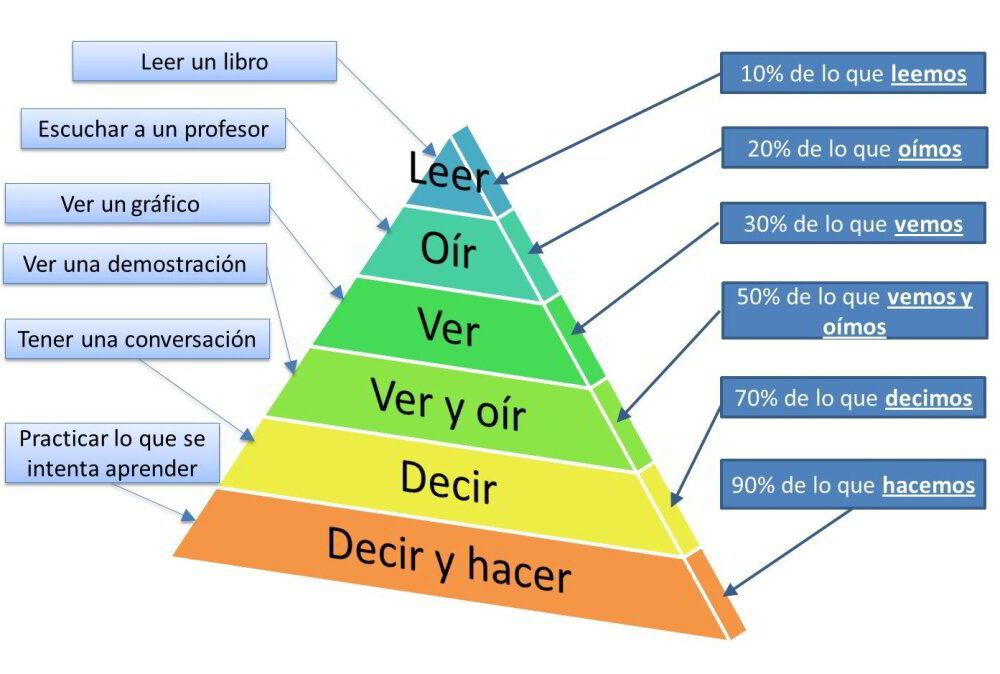
\includegraphics[width=1\linewidth]{images/pareja34_image2}
\figcaption{Cono del aprendizaje. Fuente: http://bitly.ws/po5B}

\end{minipage}
\end {flushleft}

En la figura uno podemos observar con mayor granularidad las primeras dos fases, planteadas con anterioridad, mediante el Cono del Aprendizaje de Edgar Dale. En el cono se indica qué tan eficiente será nuestro aprendizaje dependiendo del nivel de exposición con un tema mediante diferentes medios. Podemos observar que cuanto más una persona se involucra e interactúa con la información, más eficiente en porcentaje será su aprendizaje. Esto, por supuesto, considerando las diferentes formas en que un individuo puede captar la información y llegue a ser susceptible e influenciado por esta.

No debemos olvidar que cuanto mayor conocimie-
nto y claridad tengamos sobre las distintas técnicas de estudio existentes, con mayor facilidad podremos seleccionar la más adecuada a nuestra situación para así poder adaptarla y personalizarla. Aprender a estudiar sacándole partido a las capacidades personales es muy parecido a un entrenamiento físico: hace falta voluntad, un buen entrenador y constancia. Si no conocemos la manera de hacerlo no llegaremos a tener buenos resultados. Hay que querer, pero también saber.

En resumen, se puede contar con las mejores técnicas de estudios, pero el rendimiento académico se ve afectado por innumerables factores, por ejemplo, de un estudiante a otro puede variar aunque se esté utilizando la misma metodología. Se ha generalizado la idea de que los buenos hábitos de estudio influyen considerablemente en los resultados del aprendizaje, pero no hay que confundir los hábitos de estudio con las técnicas de estudio. Ambos coadyuvan a la eficiencia en el aprendizaje y son necesarios si lo que se quiere es progresar y así poder sacar el máximo provecho al aprendizaje.

\hypertarget{conclusiones-3}{%
\section{Conclusiones}\label{conclusiones-3}}

\begin{itemize}
\item
  Aprender es parte intrínseca de nuestra vida y necesitamos encontrar la mejor manera de hacerlo, llevar una planificación estructurada nos facilitará el proceso y nos beneficiará en la eficiencia del mismo. La actitud durante el aprendizaje es prioridad para obtener buenos resultados, si estamos interesados en aprender aplicaremos bien las técnicas de estudio para sacar el mejor provecho.
\item
  Debemos conocernos para identificar las prácticas que mejor se adecuen a nuestra forma de aprender y así tener claro cómo personalizar las técnicas de estudio que deseamos aplicar. Al tener una planificación estructurada podremos también generar material que nos servirá para enseñar a otros y transmitir eficientemente el conocimiento adquirido.
\end{itemize}

\hypertarget{referencias-6}{%
\section*{Referencias}\label{referencias-6}}
\addcontentsline{toc}{section}{Referencias}

\begin{itemize}
\item
  {[}1{]} {[}Gómez, Montserrat.{]}{[}Técnicas de estudio y estrategias de aprendizaje{]}. Recuperado de: \url{http://bitly.ws/po5v}. {[}Último acceso: marzo 2022{]}.
\item
  {[}2{]} {[}Martínez Otero, Valentín y Torres, Liliana{]}{[}Aná-
  lisis de los hábitos de estudio en una muestra de alumnos universitarios. Revista Iberoamericana de educación{]}. Recuperado de: \url{http://bitly.ws/po5x}. {[}Último acceso: marzo 2022{]}.
\item
  {[}3{]} {[}Dale, Juan{]}{[}El cono de Edgar Dale ¿dejamos de leer?{]}. Recuperado de: \url{http://bitly.ws/po5B}. {[}Último acceso: marzo 2022{]}.
\end{itemize}

\end {multicols}
\medskip
\HRule
\medskip

\begin{center}
\includegraphics[width=1\linewidth]{images/publicidad7} \end{center}

\hypertarget{pareja35}{%
\chapter{El desafio del docente virtual}\label{pareja35}}

\begin{center}
\includegraphics[width=1\linewidth]{images/pareja35_image1} \end{center}

\begin {multicols}{2}

\hypertarget{introducciuxf3n-4}{%
\section{Introducción}\label{introducciuxf3n-4}}

El docente es una figura muy importante para una sociedad moderna, cuyo objetivo primordial es el de formar compañeros profesionales de sectores de todas las índoles. Una de las responsabilidades de cada docente (entre muchas otras), es la de mantenerse actualizado en relación a su área de estudio y los grandes avances que puede presentar con el tiempo. Es por esto que de forma sistemática se realiza una actualización continua de docentes, para integrar los conocimientos recientes y preservar la calidad educativa.

La pandemia de COVID-19 evidenció que el sistema de actualización docente actual se queda atrás ante un mundo que avanza a pasos agigantados, que no da la prioridad suficiente al aprendizaje de temas que van más allá de lo académico, como lo son el uso de nuevas tecnologías que apoyen la docencia y la aplicación de métodos que faciliten el aprendizaje del estudiante remoto.

La labor de los docentes hoy en día se ha vuelto más que nunca fundamental para que los estudiantes aprendan y logren sobreponerse a cualquier obstáculo que les impida aprender, esto debido a la pandemia que estamos viviendo. Muchos docentes estaban acostumbrados a un sistema convencional de dar clases, incluso algunos sin saber mucho de tecnología, ahora mismo se ven obligados más que nunca a aprender otras técnicas muy útiles al impartir lecciones. Se podría decir que antes era de suma importancia la actualización continua del docente, pero ahora es más que obligatorio.

La formación continua juega un papel muy importante, ya que cada vez más la sociedad demanda una educación de calidad. Es sabido que la formación continua en el ámbito educativo ya sea que se tenga experiencia laboral o no, siempre es una buena opción para mantenerse actualizado como trabajador y mejorar nuestras competencias; Partiendo de esto y sabiendo que los docentes tienen en sus manos la misión de formar a la sociedad del futuro es necesario tener esta constante actualización de conocimiento, acá podemos ver tres razones por las cuales los docentes en la actualidad se ven obligados a una actualización.

\begin{itemize}
\tightlist
\item
  Los cambios en la tecnología
\item
  La evolución de los métodos educativos
\item
  La disminución del índice de rotación de personal
\end{itemize}

Estas son unas de las principales razones, el desafío que se tiene como docente va aumentando debido a que estamos viviendo en unos tiempos y sociedad muy cambiante no solo generacional también lo vemos en la tecnología, vemos como las situaciones que vivimos en algunas ocasiones nos hacen replantearnos en la forma que realizamos las cosas en este caso la educación nos está afectando a todos, más a los que tienen que hacer partes prácticas y que en algunas ocasiones son muy críticas o delicadas.

De forma más específica, algunos de los nuevos retos a los que los docentes se han visto expuestos son la falta de un método de enseñanza en espacios virtuales que permita tanta expresividad como un pizarrón, la dificultad de mantener la atención del estudiante, la naturaleza inestable de la comunicación virtual con la totalidad del alumnado, la traslación de evaluaciones al terreno virtual, entre otros.

Las plataformas digitales también son algo bueno para la educación, pues permiten almacenar las lecciones impartidas para la futura consulta del estudiante, facilitan la publicación del material auxiliar para el pre y el post de las clases, proveen una o varias vías de comunicación con el docente. Sin embargo, estas plataformas tan poderosas requieren una capacitación que no es impartida y se deja en manos del docente aprender a utilizarlas y aprovecharlas en su totalidad. Por supuesto ha habido docentes que a pesar del cambio repentino se han podido adecuar, todos hemos tenido un docente que aprovecha el espacio digital para enriquecer e impartir de forma excelsa su lección, pues no todo son malas noticias al hablar de clases virtuales. Las clases virtuales como muchas otras actividades también se han beneficiado de su aplicación a distancia, en tanto que no es necesario una presencialidad, una gran noticia para docentes y alumnos que se encuentran lejos del centro educativo.

Debido a esto se debe invertir desde ya en incentivar al docente a que se capacite constanteme-
nte apoyándolo en todas las áreas necesarias, dándole todas las herramientas necesarias y orientando a los que no saben por dónde comenzar, ya que en los distintos niveles de educación existen herramientas específicas para impartir las clases. No sabemos hasta cuando durará esta situación que estamos viviendo actualmente, pero nos ha permitido dar un gran salto en lo que es la educación virtual y es el tiempo exacto donde debemos aprovechar a poder aprender a adaptarnos a las distintas situaciones que puedan ocurrir.

\begin {flushleft}
\noindent\begin{minipage}[c]{\columnwidth}
\centering

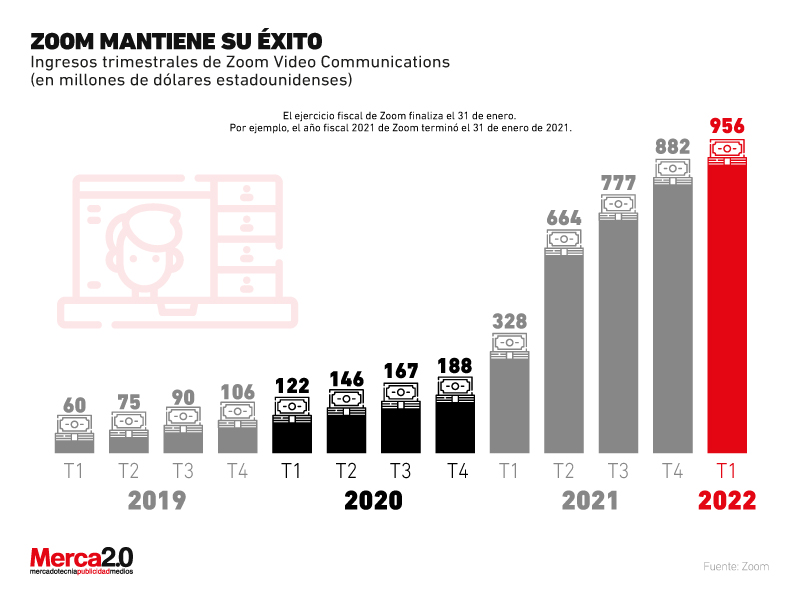
\includegraphics[width=1\linewidth]{images/pareja35_image2}
\figcaption{Facturación trimestral de Zoom. Fuente: http://bitly.ws/qp9t}

\end{minipage}
\end {flushleft}

En algunos países han pasado casi 2 años de educación virtual, aun así, con la falta de medidas eficaces para proteger la salud de los integrantes de la comunidad educativa, resulta inviable retomar una educación presencial. Teniendo esto en cuenta, sería idóneo un plan de preparación docente con enfoque en herramientas de enseñanza que van desde la impartición de lecciones magistrales hasta la comunicación efectiva que tanto beneficia al alumnado.

\hypertarget{conclusiones-4}{%
\section{Conclusiones}\label{conclusiones-4}}

\begin{itemize}
\tightlist
\item
  El docente está obligado a una actualización constante, debido al cambio continuo que existe en el mundo y más en la actualidad por la situación que estamos viviendo hablando de la pandemia
\item
  Se debe establecer, en este caso con el precedente de la pandemia, métodos alternativos para la educación a distancia con todas las conclusiones que ya hemos sacado de la situación actual.
\item
  Las vías de comunicación oficiales con el alumno deberían tener un horario de atención concreto y suficiente para el alumnado, esto pensado en delimitar el horario de trabajo del docente.
\end{itemize}

\hypertarget{referencias-7}{%
\section*{Referencias}\label{referencias-7}}
\addcontentsline{toc}{section}{Referencias}

\begin{itemize}
\item
  {[}1{]} {[}Riesco, Sofía{]}{[}Formación continua ¿presencial, distancia u online?{]}. Recuperado de: \url{http://bitly.ws/po6g}. {[}Último acceso: febrero 2022{]}.
\item
  {[}2{]} {[}Rodriguez Vite, Higor{]}{[}Importancia de la formación de los docentes en las instituciones educativas{]}. Recuperado de: \url{http://bitly.ws/po6k}. {[}Último acceso: febrero 2022{]}.
\item
  {[}3{]} {[}Nereida Josefina Valero-Cedeño, Nereida Josefina, Castillo-Matute, Ana Lisseth, Rodríguez-
  Pincay, Ronny, Padilla-Hidalgo y Merridy, Cabrera-
  Hernández, Maritza{]}{[}Retos de la educación virtual en el proceso enseñanza aprendizaje durante la pandemia de Covid-19{]}. Recuperado de: \url{http://bitly.ws/po6p}. {[}Último acceso: marzo 2022{]}.
\end{itemize}

\end {multicols}
\medskip
\HRule
\medskip

\hypertarget{mariomorales}{%
\chapter{Análisis de dificultades para la educación virtual y propuesta de mejoras de los estudiantes de la escuela de ciencias y sistemas de la USAC}\label{mariomorales}}

\begin{center}
\includegraphics[width=1\linewidth]{images/mMorales_image1} \end{center}

\begin {multicols}{2}

\hypertarget{resumen-1}{%
\section{Resumen}\label{resumen-1}}

Debido a la situación actual del mundo suscitada por la pandemia COVID 19, la educación virtual ha tomada un gran auge; un ejemplo de ello es la utilización de esta modalidad en la Escuela de Ciencias y Sistemas de la USAC. Para conocer la situación actual y oportunidades de mejora en dicha escuela se creó un instrumento de evaluación docente basado en prácticas realizadas por 2 de las mejores universidades a nivel global. El objetivo del estudio es contribuir a mejorar el modelo didáctico docente de educación virtual de la escuela de Ciencias y Sistemas mediante el estudio de la situación actual del mismo. El estudio se realizó con una encuesta enviada a través de correo con ayuda del DTT (Desarrollo de transferencia tecnológica) a los estudiantes de la escuela respecto a los cursos del área profesional, obteniendo 430 respuestas. Los resultados mostraron que los catedráticos graban sus clases y poseen dominio en la utilización de Google Meet, y UEDi. Por otra parte, se encontró que algunos catedráticos no realizan actividades complementarias.

\hypertarget{palabras-clave-1}{%
\section{Palabras clave}\label{palabras-clave-1}}

UEDi, Meet, COVID-19, E-learning, actividades complementarias, educación superior

\hypertarget{introducciuxf3n-5}{%
\section{Introducción}\label{introducciuxf3n-5}}

En la actualidad, la pandemia de COVID-2019 ha trastocado por completo la educación a nivel nacional. En 2020 y 2021, todas las instituciones educativas se vieron forzadas a renovar sus modelos educativos a un medio remoto para reducir los potenciales contagios. La Escuela de Ciencias y Sistemas (ECYS) de la USAC es un claro ejemplo de ello al brindar todas las clases a través de videoconferencias y utilizar una plataforma virtual (UEDi) para compartir material, calificar tareas, dejar proyectos, etc.

Sin embargo, este cambio de medio hacia la virtualidad conlleva un gran desafío si se pretende mantener la calidad educativa. La educación virtual no consiste únicamente en digitalizar los contenidos impartidos, sino que representa un cambio en la manera de enseñar. Las sesiones virtuales deben ser amenas para todos, a la vez que se deben realizar actividades para garantizar la correcta abstracción de los temas.

El presente trabajo revisa el desempeño de la ECYS respecto al cambio de clases virtuales a través de un instrumento distribuido a sus alumnos. Posteriormente, los resultados son revisados para determinar las oportunidades de mejora y por último se presenta un marco de buenas prácticas que pueden ayudar a enriquecer la calidad educativa.

\textbf{Materiales y Métodos}

\emph{Diseño:} Esta investigación se realizó con una metodología cuantitativa con un diseño de tipo no experimental.

\emph{Población y entorno:} El muestreo fue por disponibili-
dad.

\emph{Intervenciones:} El instrumento es una encuesta utilizada en esta investigación, el cual fue de elaboración propia con base en buenas prácticas en educación virtual empleadas en las universidades norteamericanas MIT y Harvard. Además, se creó un marco de buenas prácticas, el cual se encuentra al final del presente documento.

Este marco está basado en las prácticas de las universidades anteriormente mencionadas

\textbf{Resultados}

En la figura 9.1 se observa que la respuesta con mayor representatividad de preguntas negativas es la pregunta 7, con un porcentaje del 26.42\%. Por lo cual podemos afirmar que algunos catedráticos deberían realizar actividades complementarias a las clases virtuales.

Además, en la figura 9.2 se aprecia la lista de las 5 secciones con peor nota las cuales son: Arqui 2 sec.~``N'', IPC 2 sec.~``B'', Modelación 2, Organización Computacional sec.~``A'' y Sistemas Operativos 2. Estos cursos poseen una muy buena oportunidad de mejora para asignar más actividades complementarias que ayuden a los estudiantes a comprender los contenidos brindados.

\textbf{Discusión}

Actualmente se cuenta con la plataforma virtual docente UEDi en donde se comparte cualquier material oficial. Las clases son impartidas a través de Google Meet, la cual es una buena plataforma como podemos ver en el cuadrante de Gartner en el cual posee una posición buen como challenger (ver figura 9.3). Esta plataforma integra las cuentas de correo oficiales de los alumnos para agendar el horario lo cual facilita su uso.

Conociendo cual es el estado actual del modelo docente, listaremos oportunidades de mejora para el mismo. La primera oportunidad de mejora es compartir siempre los materiales y apuntes presentados en las clases virtuales por los docentes, situación que se refleja en ciertos cursos y secciones específicas de la carrera.

Actualmente Google Meet permite grabar las sesiones para que el alumno la pueda revisar posteriormente las lecciones impartidas en el día de clase, pero también es recomendable compartir cualquier apunte realizado en clase esto utilizando la plataforma oficial UEDi. A veces es más sencillo examinar un diagrama para entender una explicación, que revisar la sesión completa.

La siguiente oportunidad para docentes y tutores académicos es evitar leer las presentaciones. Hay que recordar que las presentaciones son solo una herramienta que facilita resaltar ciertos puntos al explicar un tema.

Otro punto importante, es buscar maneras de hacer más dinámicas las clases en específico la validación del conocimiento del estudiante al final de cada sesión. Actualmente se cuenta con diversas herramientas didácticas gratuitas en línea que nos ayudan a hacer diversas actividades didácticas en clases virtuales.

Los resultados muestran que se necesitan agregar más actividades complementarias al plan de estudio con el fin de ayudar a la comprensión de los temas y darles dinamismo a las clases (ver figura 9.1).

\textbf{Agradecimientos}

La investigación fue llevada a cabo con el apoyo de la dirección del DTT (Desarrollo de Transferencia Tecnológica) y la Escuela de Ciencias y Sistemas.

\hypertarget{referencias-8}{%
\section*{Referencias}\label{referencias-8}}
\addcontentsline{toc}{section}{Referencias}

\begin{itemize}
\item
  {[}1{]} {[}González, Rocío{]}{[}Clases virtuales en contextos de emergencia: COVID-19{]}. Recuperado de: \url{http://bitly.ws/qriQ}. {[}Último acceso: marzo 2021{]}.
\item
  {[}2{]} {[}Revista ingeniería y ciencia{]}{[}Deserción estudiantil en las Universidades de Guatemala y en la Universidad Rafael Landívar{]}. Recuperado de: \url{http://bitly.ws/qrj9}. {[}Último acceso: marzo 2021{]}.
\item
  {[}3{]} {[}Gartner{]}{[}Gartner Magic Quadrant for Meeting Solutions{]}. Recuperado de: \url{http://bitly.ws/qrjc}. {[}Último acceso: marzo 2021{]}.
\item
  {[}4{]} {[}Hernández, Verónica{]}{[}Haciendo la transición de educación presencial a educación virtual{]}. Recuperado de: \url{http://bitly.ws/qrje}. {[}Último acceso: marzo 2021{]}.
\item
  {[}5{]} {[}Organización Panamericana de la Salud{]}{[}Se confirma primer caso de COVID-19 en Guatemala{]}. Recuperado de: \url{http://bitly.ws/qrji}. {[}Último acceso: marzo 2021{]}.
\item
  {[}6{]} {[}Harvard University{]}{[}Teach Remotely{]}. Recupe-
  rado de: \url{http://bitly.ws/qrjj}. {[}Último acceso: abril 2021{]}.
\item
  {[}7{]} {[}Massachusetts Institute of Technology{]}{[}Teach Remote{]}. Recuperado de: \url{http://bitly.ws/qrjp}. {[}Último acceso: mayo 2021{]}.
\item
  {[}8{]} {[}Morales Saldarriaga, Juan Carlos{]}{[}Tweets sobre e-Learning: Reflexiones y definiciones sobre educación virtual{]}. Recuperado de: \url{http://bitly.ws/qrjr}. {[}Último acceso: abril 2021{]}.
\end{itemize}

\begin {flushleft}
\noindent\begin{minipage}[c]{\columnwidth}
\centering

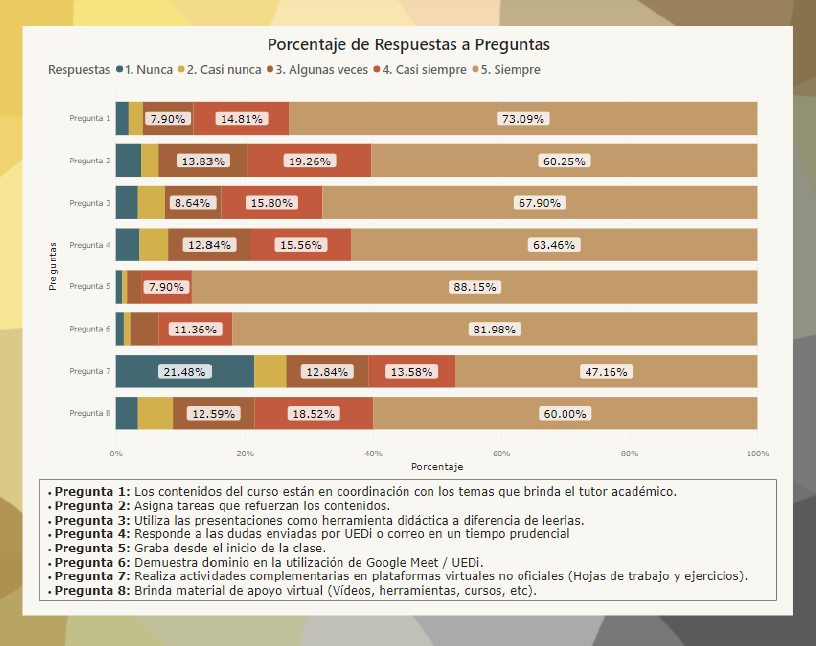
\includegraphics[width=1\linewidth]{images/mMorales_image2}
\figcaption{Gráfico de barras acumuladas de porcentajes de respuestas a preguntas del instrumento de evaluación. Fuente: Elaboración propia}

\end{minipage}
\end {flushleft}

\begin {flushleft}
\noindent\begin{minipage}[c]{\columnwidth}
\centering

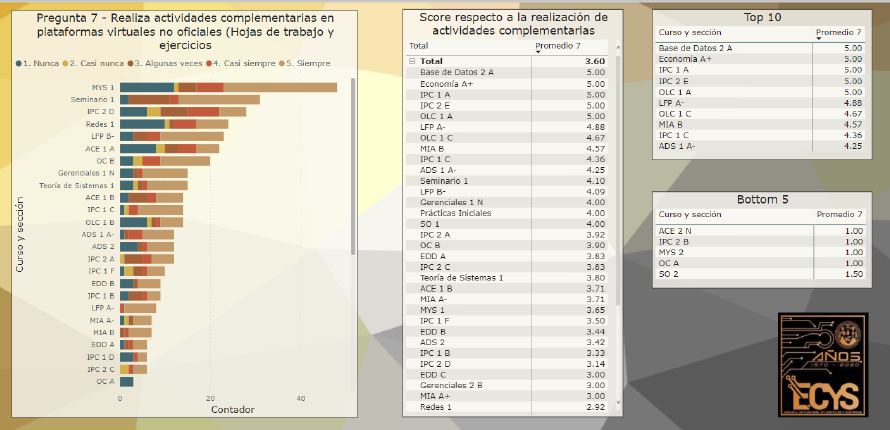
\includegraphics[width=1\linewidth]{images/mMorales_image3}
\figcaption{Dashboard pregunta no. 7 sobre Actividades complementarias. Fuente: Elaboración propia}

\end{minipage}
\end {flushleft}

\begin {flushleft}
\noindent\begin{minipage}[c]{\columnwidth}
\centering

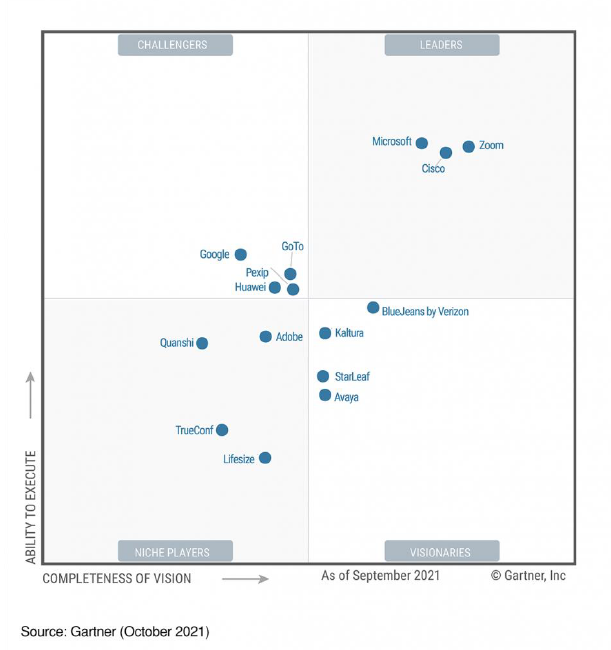
\includegraphics[width=1\linewidth]{images/mMorales_image4}
\figcaption{Cuadrante mágico de Gartner de plataformas para reuniones. Fuente: Gartner}

\end{minipage}
\end {flushleft}

\begin {flushleft}
\noindent\begin{minipage}[c]{\columnwidth}

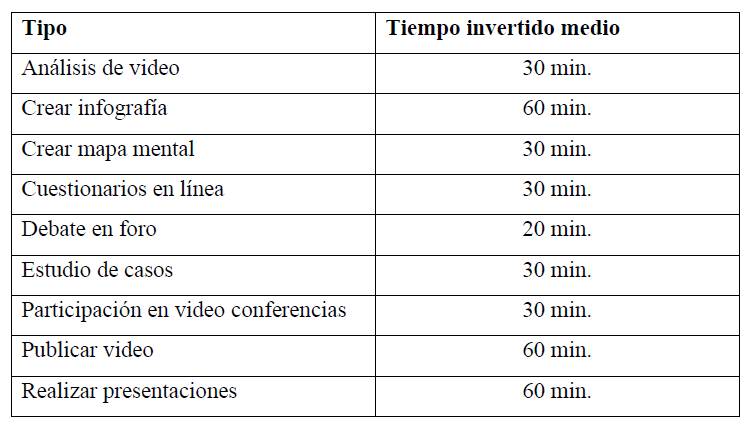
\includegraphics[width=1\linewidth]{images/mMorales_image5}
Tabla 9.1: Actividades en modalidad virtual. Fuente: eLearning Masters -- Universidad Galileo. Recuperado de: \url{http://bitly.ws/qrjH}

\end{minipage}
\end {flushleft}

\end {multicols}

\hypertarget{guippsymenendez}{%
\chapter{Evolución de las Pruebas de Conocimientos Básicos de la presencialidad a la virtualidad en época de pandemia}\label{guippsymenendez}}

\begin{center}
\includegraphics[width=1\linewidth]{images/gMenendez_image1} \end{center}

\begin {multicols}{2}

La Universidad de San Carlos de Guatemala USAC, desde sus inicios se ha preocupado en lograr una calidad académica abriendo sus puertas como única universidad pública del país, se han realizado diversos esfuerzos en formar a los futuros profesionales del país. La USAC, así como muchas universidades tanto del país como del mundo entero, han tenido que enfrentarse a retos de diversa índole, entre ellos epidemias devastadoras que han impactado en su funcionamiento cotidiano, han logrado sobrevivir y continuar con su misión aún a puertas cerradas.

Ante la emergencia por las condiciones que prevalecen en el país relacionada con el avance y efectos de la pandemia por la que atraviesa el mundo entero, las instituciones educativas se vieron en la necesidad de implementar sistemas no presenciales basados en plataformas digitales para cumplir con el proceso de enseñanza aprendizaje. Por lo que, la educación en línea es una de las actividades que se ha fortalecido durante el confinamiento, las aulas físicas se convirtieron en espacios virtuales, proyectándose a un público disperso geográficamente.

Las estimaciones de UNESCO IESALC, muestran que el cierre temporal afecta aproximadamente a unos 23.4 millones de estudiantes de educación superior y a 1.4 millones de docentes en América Latina y el Caribe, esto representa, aproximadamente, más del 98\% de la población de estudiantes y profesores de educación superior de la región.

La USAC ha asumido el reto de implementar la educación en línea, reformulando procesos académicos y administrativos en beneficio de la población estudiantil y sociedad en general, permitiendo que gran parte de la población tenga acceso a la educación. Otro reto asumido por la USAC ha sido implementar el proceso de ingreso en línea. Según el Artículo 28 del Reglamento del SUN, el encargado de realizar las Pruebas de Conocimientos Básicos PCB es el Sistema de Ubicación y Nivelación SUN, el cual desde el año 2000 ha venido realizándolas de forma presencial.

En el año 2020 se implementan las PCB de forma virtual, con la finalidad de evitar aglomeraciones en su aplicación y de esta manera garantizar el proceso de ingreso a los aspirantes que deseen ingresar a la USAC para el ciclo 2021. Se implementó un programa de aplicación de PCB en el cual los aspirantes desde cualquier dispositivo electrónico con conexión a internet (computadora de escritorio, Tablet, laptop, teléfono inteligente, entre otros) tienen acceso a la misma desde cualquier lugar en donde se encuentren.

Las personas han tenido que reorganizar su vida cotidiana para ajustarse al confinamiento, muchas personas desplazadas lejos de sus familias en el extranjero, se han quedado varados esperando a poder regresar a sus países. Con la implementación de las PCB de forma virtual en el año 2020, se logró que muchos aspirantes que se encontraban varados fuera del país tuvieran acceso a realizar las pruebas. Según la UNESCO IESALC, el 17 de marzo de 2020, ya se había llegado a una cifra de 21.7 millones de estudiantes y 1.3 millones de docentes afectados por los cierres temporales.

En la actualidad las TIC´s han revolucionado el mundo, modificando los niveles de comunicación, es por esto, que el SUN haciendo uso de las misma, ha logrado implementar la inscripción, aplicación y entrega de resultados en línea a nivel nacional, es decir, en el campus central y en los Centros Universitarios Departamentales. (Ventura 2021) en su investigación, evidenció que el 92.8\% lo que equivale a 4,798 aspirantes de los encuestados, consideran que la implementación del proceso de ingreso en modalidad virtual ha sido de beneficio, mientras que el 7.2\% considera lo contrario.

Los beneficios que han obtenido los aspirantes a ingresar a la USAC con la implementación de las PCB en línea, han sido diversos, pudiendo mencionar entre ellos, ahorro de tiempo y recursos en la movilización física, no estar expuesto al contagio de COVID-19, poder realizar las pruebas desde cualquier lugar en donde se encuentren por medio de un dispositivo electrónico con conexión a internet, apoyo en sus trabajos relacionado a permisos para realizar las pruebas, entre otros.

\hypertarget{conclusiones-5}{%
\section{Conclusiones}\label{conclusiones-5}}

\begin{itemize}
\item
  A pesar que la pandemia ha impactado de forma totalmente abrupta, la USAC ha sabido enfrentar todos los retos logrando implementar sistemas no presenciales basados en plataformas digitales para cumplir con el proceso de enseñanza aprendizaje, aunado a esto, ha logrado romper con las barreras culturales implementando el proceso de ingreso en línea. Muchos aspirantes que se quedaron varados en el extranjero o incluso dentro del mismo país, imposibilitados a regresar a sus hogares debido al cierre de aeropuertos y fronteras, tuvieron la oportunidad de realizar sus PCB, a través de los programas de aplicación que la USAC puso a su disposición con tan solo disponer de un dispositivo electrónico con conexión a internet.
\item
  Muchos han sido los beneficios logrados con la implementación de plataformas digitales, es difícil predecir cuando terminará la actual pandemia, los efectos que ha causado han sido grandes y han dejado huella en la vida de muchos, es necesario contar con un plan de contingencia y trazar líneas fundamentales de salida ante nuevas crisis que se puedan presentar.
\end{itemize}

\hypertarget{referencias-9}{%
\section*{Referencias}\label{referencias-9}}
\addcontentsline{toc}{section}{Referencias}

\begin{itemize}
\item
  {[}1{]} {[}UNESCO IESALC{]}{[}Covid-19 y educación superior: de los efectos inmediatos al día después{]}. Recuperado de: \url{http://bitly.ws/pHJH}. {[}Último acceso: febrero 2022{]}.
\item
  {[}2{]} {[}Universidad de San Carlos de Guatemala{]}{[}Re-
  glamento del Sistema de Ubicación y Nivelación SUN{]}. {[}Último acceso: febrero 2022{]}.
\item
  {[}3{]} {[}Ventura, A{]}{[}Las TIC´s en la educación: uso de las TIC´s en el proceso de ingreso a la Universidad de San Carlos de Guatemala{]}. {[}Último acceso: febrero 2022{]}.
\end{itemize}

\end {multicols}
\medskip
\HRule
\medskip

\begin{center}
\includegraphics[width=1\linewidth]{images/publicidad12} \end{center}

\hypertarget{pareja36}{%
\chapter{Entrevistas en tiempos de pandemia}\label{pareja36}}

\begin{center}
\includegraphics[width=1\linewidth]{images/pareja36_image1} \end{center}

\begin {multicols}{2}

A continuación se abordan temas que nos dan a conocer las distintas formas y herramientas utilizadas para la elaboración entrevistas laborales en épocas de COVID-19 que dio inicio en Enero de 2020 en la ciudad de Wuhan, China.

La pandemia desarrollada por el virus SARS-CoV-2 afectó de una gran manera a la población mundial, llegando a paralizar no sólo las actividades de tipo comercial, sino también cualquier actividad en donde existiese interacción humana. Debido a esta parálisis las personas se vieron obligadas a desarrollar nuevos métodos para retomar sus vidas, siendo una de ellas el teletrabajo o trabajo remoto así como la forma en que funciona el reclutamiento de las empresas en su nuevo personal de trabajo.

Todas las empresas que adoptaron el medio de trabajo, que se denomina Home Office, hacen uso de plataformas públicas para conectar con las personas que quieren aplicar para algún puesto de trabajo que ofrezcan, la situación está en que habiendo muchas es posible que todos hayan elegido una al azar y no se hayan percatado de si hay alguna plataforma que sea mejor o si la que están usando tiene características que les serían útiles pero no está al tanto de estas.

Antes de la crisis por la pandemia del Covid-19 en España solo un 40\% de entrevistas de trabajo se realizaban de forma virtual, sin embargo dicha crisis ha incrementado la necesidad de crear unos formatos de trabajo de forma virtual por lo que el reclutamiento de personal ha ido incrementando sin cesar. La implementación del teletrabajo se ha reflejado en el uso de plataformas como Zoom o Google Meet para las conferencias de la mayoría de la fuerza de trabajo por lo que ha crecido la necesidad de contar con personal profesional digital.

La transformación digital ha hecho que las empresas cambien sus métodos para la selección del nuevo personal de trabajo, el software de reclutamiento para la selección del mismo puede variar y entre algunos de ellos podemos encontrar los siguientes: Teams, Slack, Skype, Google Meet.

Con el avance de la pandemia las estadísticas muestran que el uso de estas herramientas se disparó por lo que cada día son más las empresas que requieren de dicho software para el reclutamiento de su personal. También es importante mencionar que ante este avance cada día es mayor el número de personas que se adaptan a la utilización de dicho software en su vida cotidiana ya que es un requisito para poder optar a aplicar a un puesto de trabajo.

Es importante mencionar que a la hora de entrevistar a las personas es importante preguntar cómo mezclan su vida cotidiana con su vida laboral ya que es imprescindible que exista un plan de conciliación familiar así como evaluar la honestidad y calidad humana de cada candidato.

\begin {flushleft}
\noindent\begin{minipage}[c]{\columnwidth}
\centering


\includegraphics[width=1\linewidth]{images/pareja36_image2}
\figcaption{Representación gráfica de comunicación en pandemia. Fuente: http://bitly.ws/qp9v}

\end{minipage}
\end {flushleft}

También hay que tomar en cuenta que las entrevistas en línea pueden abrir oportunidad a mucha gente para aplicar a puestos de trabajo que se encuentren lejos de sus residencias, ya que últimamente los medios de movilización al ser de acceso público cualquier persona puede exponerse ante el virus, no solo eso sino que también no todos cuentan con medios propios de movilización, ya sean automóviles o motocicletas. Además que hoy en día se puede acceder a internet y conseguir un dispositivo electrónico que le permita acceder a distintas herramientas de interconexión social.

\begin {flushleft}
\noindent\begin{minipage}[c]{\columnwidth}
\centering


\includegraphics[width=1\linewidth]{images/pareja36_image3}
\figcaption{El kit para realizar con éxito una entrevista de trabajo on-line. Fuente: http://bitly.ws/qp9w}

\end{minipage}
\end {flushleft}

\hypertarget{conclusiones-6}{%
\section{Conclusiones}\label{conclusiones-6}}

\begin{itemize}
\tightlist
\item
  Lo bueno de estas entrevistas en línea es que incluso una persona puede aplicar a un trabajo en el extranjero sin las preocupaciones de gestión de vuelos y hoteles
\item
  Las entrevistas de trabajo en línea han abierto oportunidades para muchas personas que buscan oportunidades laborales que se encuentran lejos de sus residencias.
\item
  Sin duda alguna y a pesar de la tragedia que ha significado la pandemia del COVID-19 para las personas, es un hecho que ha contribuido a la actualización de las personas y las empresas en general.
\item
  Las personas se actualizan en temas de tecnología para poder optar por un puesto laboral
\end{itemize}

\hypertarget{referencias-10}{%
\section{Referencias}\label{referencias-10}}

\begin{itemize}
\item
  {[}1{]} {[}López Escalante, Gabriela{]}{[}Entrevista de trabajo por Zoom: así es la búsqueda de empleo en pandemia{]}. Recuperado de: \url{http://bitly.ws/po7C}. {[}Último acceso: febrero 2022{]}.
\item
  {[}2{]} {[}Peinado, Félix{]}{[}Así son las entrevistas de trabajo post COVID-19{]}. Recuperado de: \url{http://bitly.ws/po7D}. {[}Último acceso: febrero 2022{]}.
\item
  {[}3{]} {[}Weed, Julie{]}{[}Como triunfar en una entrevista laboral por internet{]}. Recuperado de: \url{http://bitly.ws/po7E}. {[}Último acceso: febrero 2022{]}.
\end{itemize}

\end {multicols}
\medskip
\HRule
\medskip

\begin{center}
\includegraphics[width=1\linewidth]{images/publicidad8} \end{center}

\hypertarget{pareja38}{%
\chapter{El presente del trabajo del futuro}\label{pareja38}}

\begin{center}
\includegraphics[width=1\linewidth]{images/pareja38_image1} \end{center}

\begin {multicols}{2}

\hypertarget{introducciuxf3n-6}{%
\section{Introducción}\label{introducciuxf3n-6}}

La pandemia ha tomado auge en los últimos años a medida que el COVID-19 ha evolucionado y se ha visto afectado tanto en lo económicamente como dentro del ámbito organizacional dentro de las empresas, algunos datos realizados por estudios constan que actualmente hay altos grados de incertidumbre, la mayoría considera que el trabajar de manera remota ha sido un beneficio para muchos trabajadores.

El golpe recibido en el año 2020, en el inicio de la pandemia, impulsó a desarrollar programas administrativos para mantener el servicio o productos y mitigar los daños causados a empresas guatemalte-
cas. Sin embargo, cuando se creía que nuestro país no podría otorgar oportunidades laborales a distancia por la falta de desarrollo y el miedo al cambio que invadía el pensamiento de muchas empresas, se establecieron nuevas formas de trabajo para mantener la integridad física de los empleados y no perder la integridad económica de las empresas. Las maneras de trabajar han evolucionado de tal forma que estas han descubierto grandes ventajas, al igual que muchos estudiantes, teniendo la capacidad de organizar su tiempo de una manera que no interrumpan sus estudios y seguir cumpliendo sus labores de la mejor manera.

La manera remota ha sido de gran ayuda para muchos trabajadores, también se considera importante para algunos trabajadores que se retorne a la manera presencial, ya que muchas de estas organizaciones dependen económicamente de esta modalidad, así mismo, se toma en cuenta en cómo ha afectado en la economía mundial la pandemia, estos datos pueden ser extraídos del Banco Mundial que revela una manera predictiva de obtener las estadísticas y lo que se prevé para los siguientes años, así como obtener datos de los años pasados.

\hypertarget{artuxedculo-2}{%
\section{Artículo}\label{artuxedculo-2}}

En cuanto a la productividad en las organizaciones se han visto obligados o en la necesidad de trabajar en diferentes plataformas permitiendo la comunicación remota entre los trabajadores. Según los datos de la economía mundial proporcionados por el Banco Mundial ``Se prevé que el crecimiento mundial se desacelere al 4,1 \% en 2022, como reflejo de los continuos brotes de COVID-19, la disminución del apoyo fiscal y las persistentes dificultades en las cadenas de suministro. Aunque se proyecta que la producción y la inversión en las economías avanzadas volverán a las tendencias previas a la pandemia el próximo año''.

Un estudio realizado por la empresa Talana, que analizó a casi 400 firmas respecto a la modalidad virtual y el retorno a la modalidad presencial. ``De acuerdo con la quinta versión del estudio ``Vuelta al Trabajo'' desarrollado por Talana (plataforma que digitaliza el área de recursos humanos de las empresas), el 24\% de las firmas decidió volver a tiempo completo a las oficinas en noviembre de 2021, el doble de lo registrado en el último informe de agosto pasado''. El 73\% de las empresas declaró que planea mantener el teletrabajo, en mayor o menor medida, una vez terminada la pandemia.

Entonces ¿Cuál es el futuro para el trabajo de muchos estudiantes que aspiran a ser ingenieros?, ¿Qué retos deben de superar los guatemaltecos al estar con la nueva metodología de trabajo?, estas y otras preguntas están en el futuro de empresas y trabajadores en nuestro país; sin embargo, la pandemia ha demostrado que, aunque somos un país en desarrollo que puede adaptarse, no sólo a las circunstancias sino a cubrir las necesidades de un teletrabajo.

El estudiante de la facultad de ingeniería se ha caracterizado por ser una persona esforzada, que muchas veces llega a permanecer en la universidad por varias horas durante el día, realizando proyectos individuales o en grupo, todos luchando para alcanzar una misma meta, sin embargo, el reto de poder estudiar y trabajar, tristemente era algo que muy pocos alcanzaban, por la necesidad de ayudar en su hogar, decidían ya no continuar con sus estudios universitarios. El poder alcanzar un título universitario, no se veía una meta a obtener porque la necesidad económica en el hogar guatemalteco es más fuerte que un sueño universitario.

\begin {flushleft}
\noindent\begin{minipage}[c]{\columnwidth}
\centering

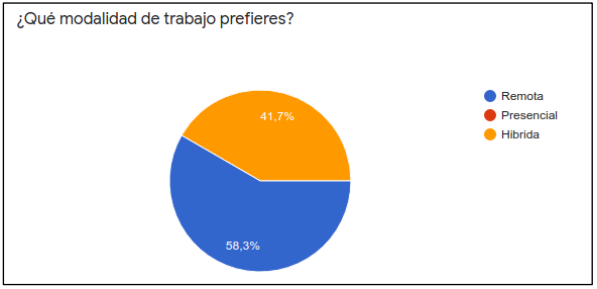
\includegraphics[width=1\linewidth]{images/pareja38_image2}
\figcaption{Modalidad de trabajo. Fuente: Elaboración propia}

\end{minipage}
\end {flushleft}

Como estudiantes, nos dimos a la tarea de consultar a los estudiantes que realizan labores remotas, por lo que los resultados en esta encuesta un 58.3\% de estos prefieren una modalidad 100\% remota mientras que el 41.7\% de los encuestados prefieren que la modalidad de trabajo sea híbrida (Figura 1).

Aunque la pandemia llegó a afectar la economía, salud y bienestar a nivel mundial, al encerrar a toda una población y estancar el movimiento normal en un país, también logró demostrar que la economía puede avanzar desde casa y esto fue una esperanza de lograr el tan anhelado sueño estudiantil.

En nuestro país el reto tecnológico, en el teletrabajo, se está superando, pero se tiene que lograr construir una cultura que pueda preservar distintas expansiones que se desee gestionar para obtener lo mejor de los empleados, nivelando las dos formas de trabajo que se están implementando, ya muchas empresas guatemaltecas poseen oficinas abiertas para poder dar opciones a los empleados, manteniendo un balance y cuidado de los trabajadores.

Dicho balance ha permitido a muchos estudiantes, puedan adquirir experiencia laboral complementando sus estudios, esta gran oportunidad no solamente ha beneficiado a nuestra población en ingeniería, si no también ha logrado ayudar a varias personas que han dejado de estudiar en distintos ciclos de estudio.

\textbf{Beneficios y ventajas del teletrabajo}

Anteriormente, se menciona que se realizó una encuesta, el cual también preguntamos algunos beneficios que pudieran mejorar la experiencia de trabajar en forma remota algunos de estos son:

\begin{itemize}
\tightlist
\item
  Ahorro de tiempo y gastos de movilidad por el tráfico generado diariamente.
\item
  Mayor comodidad y estrés que puede mejorar el nivel de vida, además de seguridad y bienestar emocional.
\item
  Flexibilidad de horarios durante el trabajo y personales.
\item
  Mayor tiempo de productividad tanto en el trabajo, como para las personas que estudian.
\item
  Apoyo económico e incentivos que algunas organizaciones dan para motivar a los empleados.
\item
  Ahorro de gastos para empresas, tales como infraestructura y servicios básicos.
\end{itemize}

\textbf{Desventajas y desafíos del teletrabajo}

Algunas de estas desventajas pueden afectar a muchas personas y el entorno tanto laboral como personal en el que interactúan diariamente, estas son algunas:

\begin{itemize}
\tightlist
\item
  Distracciones e interrupciones que pueden darse en el ambiente.
\item
  Disciplina en los horarios y cumplimiento de las tareas
\item
  Trabajar y estudiar simultáneamente
\item
  Aprender nuevas tecnologías y metodologías siendo autodidacta.
\item
  En algunos casos, el entendimiento de instruccio-
  nes.
\item
  Interacción social y la dificultad del trabajo en equipo por videollamadas o reuniones remotas.
\item
  Organización del tiempo.
\item
  El sedentarismo crece y pueden aumentar los problemas de salud físicos.
\end{itemize}

\textbf{Consejos para el entorno laboral remota:}

La adaptación al teletrabajo no es tarea fácil y depende de la personalidad de cada uno. Lo que en un primer momento puede parecer asequible, con el paso de los días puede hacerse cuesta arriba. Por esa razón, aquí exponemos una serie consejos para sacar el máximo provecho:

\begin{itemize}
\tightlist
\item
  Sé disciplinado e impone una rutina con unos horarios y unos hábitos estrictos.
\item
  Crea un espacio ordenado, cómodo y que sientas propio desde el que trabajar.
\item
  Separa las obligaciones laborales del ocio. Es decir, a determinada hora desconecta.
\item
  Evita el sedentarismo. Por ejemplo, cada cierto tiempo levántate y estira los músculos.
\item
  Habla con las personas con las que convives para que respeten tu espacio laboral.
\item
  Contacta con tus compañeros para evitar el aislamiento y facilitar el trabajo en equipo.
\end{itemize}

\hypertarget{conclusiones-7}{%
\section{Conclusiones}\label{conclusiones-7}}

\begin{itemize}
\tightlist
\item
  Como trabajadores, se debe de mantener responsabilidad y ética, esto asegurará que las empresas puedan confiar en tener esta metodología laboral.
\item
  Empresas guatemaltecas, encuentran beneficios y crecimiento económico en la pandemia provocada por Covid-19 impulsado por el teletrabajo.
\item
  La adaptación dentro del entorno laboral debe ser esencial para un equilibrio como trabajador y dentro de cualquier ambiente en que se encuentre laborando.
\end{itemize}

\hypertarget{referencias-11}{%
\section{Referencias}\label{referencias-11}}

\begin{itemize}
\item
  {[}1{]} {[}Banco Mundial{]}{[}Perspectivas económicas mundiales{]}. Recuperado de: \url{http://bitly.ws/ivUC}. {[}Último acceso: marzo 2022{]}.
\item
  {[}2{]} {[}Lanza Malavé, Rossany{]}{[}Solo un tercio de las empresas exige a sus trabajadores esquema de vacunación completa para volver en mod presencial{]}. Recuperado de: \url{http://bitly.ws/po8G}. {[}Último acceso: marzo 2022{]}.
\item
  {[}3{]} {[}Iberdrola S.A.{]}{[}Consejos para teletrabajar{]}. Recuperado de: \url{http://bitly.ws/po8M}. {[}Último acceso: marzo 2022{]}.
\item
  {[}4{]} {[}Iberdrola S.A.{]}{[}El teletrabajo o cómo aunar conciliación familiar y productividad{]}. Recuperado de: \url{http://bitly.ws/po8Q}. {[}Último acceso: marzo 2022{]}.
\end{itemize}

\end {multicols}
\medskip
\HRule
\medskip

\begin{center}
\includegraphics[width=1\linewidth]{images/publicidad16} \end{center}

\hypertarget{pareja40}{%
\chapter{Desarrolladores, la indispensabilidad de la década}\label{pareja40}}

\begin{center}
\includegraphics[width=1\linewidth]{images/pareja40_image1} \end{center}

\begin {multicols}{2}

\hypertarget{introducciuxf3n-7}{%
\section{Introducción}\label{introducciuxf3n-7}}

El término ``Era Digital'' tuvo un impacto diferente a partir del año 2021, el traslado del mundo presencial al mundo digital se volvió imprescindible en lugar de tomar su tiempo para poder implementarse paulatinamente a causa de la pandemia que inicio a principios del año 2020 hasta la fecha. La demanda aumentada de desarrolladores reflejó la urgencia de trasladar todo a formato digital, ya sea para trasladar algo existente, poder iniciar una idea emprendedora o arreglar algo ya desarrollado.

Por otro lado, la demanda aumentada pudo satisfacerse por un mismo comportamiento en la oferta de desarrolladores, pero el problema ahora se encuentra en saber cómo escoger a los candidatos ideales. Los reclutadores cambiaron sus métodos de reclutamiento y, ahora, los desarrolladores deben adaptarse a estos nuevos métodos para adaptarse a la transformación del mercado laboral.

\textbf{Desarrolladores}

La mayoría de desarrolladores aprenden a programar en la universidad o en la escuela, pero más de un tercio aprenden por su cuenta, esto ha obligado a las empresas a replantear sus métodos y estrategias de contratación, ofreciendo incluso oportunidades de capacitación interna, por lo que ya no es estrictamente necesario poseer un título universitario, ya que la experiencia en desarrollo está siendo muy tomada en cuenta.

La enorme escasez de desarrolladores ha represen-
tado un aumento en los salarios de los desarrolladores de software y ha convertido al sector de TI (Tecnologías de la información) en el sector mejor pagado. Los salarios varían respecto al país, siendo Estados Unidos, Suiza y Canadá los países más lucrativos para un desarrollador.

Los desarrolladores y reclutadores usualmente tienen opiniones diferentes respecto a las habilidades que desean adquirir o contratar. Según una encuesta, para este 2022, entre las habilidades que los desarrolladores están más interesados en aprender se encuentran: AI/Machine Learning, Web Development y Game Development.

Respecto a los lenguajes de programación, la cantidad de desarrolladores que conocen los lenguajes que los reclutadores buscan es muy consistente. Esto quiere decir que la mayoría de desarrolladores son conscientes de la demanda de lenguajes de programación, entre los lenguajes más solicitados se encuentran: JavaScript, Java y Python.

\begin {flushleft}
\noindent\begin{minipage}[c]{\columnwidth}
\centering

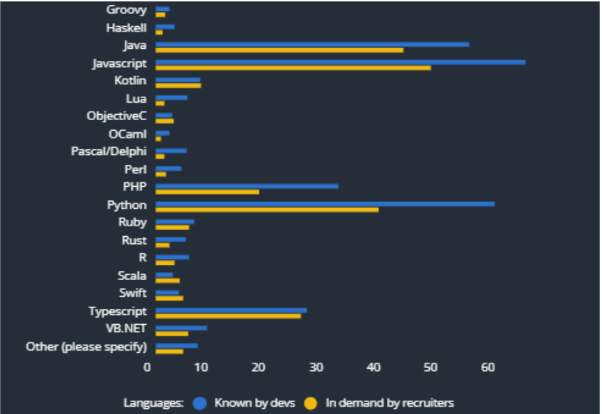
\includegraphics[width=1\linewidth]{images/pareja40_image2}
\figcaption{Encuesta CoderPad y CodinGame. Fuente: http://bitly.ws/qp9y}

\end{minipage}
\end {flushleft}

\textbf{Reclutadores}

Actualmente es un ``mercado de compradores'' para trabajos en el área de sistemas, en el que los desarrolladores pueden elegir dónde quieren trabajar no solo en qué empresa sino también en la rama de su preferencia. El desafío para los reclutadores es conquistarlos, y esto significa ofrecer salarios competitivos. A esto se suma la demanda de perfiles de desarrollador e ingeniero de software con opción a trabajar en remoto se aumentan, la modalidad de teletrabajo supone ciertas ventajas tanto para las empresas como para los trabajadores.

La cultura es la primera aproximación que toman los reclutadores, es importante para ellos dejarle claro a los desarrolladores que estos tienen flexibilidad en el área de trabajo, pueden ser ellos mismos, son importantes para el equipo y darles la oportunidad de crecimiento. Crear un ambiente agradable incluso afuera de la oficina para que los desarrolladores recomienden la empresa a sus contactos.

El siguiente paso es que la empresa comprenda a detalle el papel de los desarrolladores, es ya bien sabido que cuando se contrata a un desarrollador normalmente se le denomina ``el experto'' en el área de tecnología, pero se debe saber exactamente qué está haciendo el desarrollador en esta empresa y acordarle tareas de su área, no darle la carga de varias áreas pensando que este llego para resolver todos los problemas. El reclutador debe dejar de forma clara a la empresa que es lo que esta busca.

En el lado de los negocios las también existe una tendencia a las habilidades más demandadas, aun con la bien conocida escasez de desarrolladores full-stack y back-end, las 3 habilidades más buscadas por los reclutadores son: DevOps, Inteligencia Artificial y Machine Learning.

Una tendencia para el próximo año es que los métodos de contratación están evolucionando hacia los llamados criterios más objetivos, en particular a través de evaluaciones de habilidades y entrevistas técnicas prácticas.

Los desarrolladores ahora tienen más libertad para decidir qué ofertas de trabajo aceptar, la mayoría busca compensaciones satisfactorias, oportunidades de crecimiento y trabajo remoto, mientras que las empresas deben adaptarse a las demandas, de otra forma no podrán garantizar que su desarrollo tecnológico y posición en el mercado no se estanque.

\begin {flushleft}
\noindent\begin{minipage}[c]{\columnwidth}
\centering

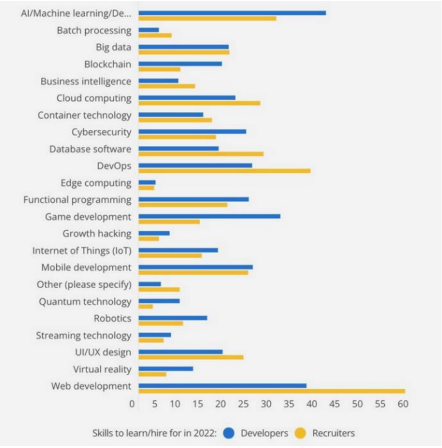
\includegraphics[width=1\linewidth]{images/pareja40_image3}
\figcaption{Encuesta CoderPad y CodinGame. Fuente: http://bitly.ws/qp9y}

\end{minipage}
\end {flushleft}

\hypertarget{referencias-12}{%
\section{Referencias}\label{referencias-12}}

\begin{itemize}
\item
  {[}1{]} {[}Codingame{]}{[}Codingame coderpad tech hiring survey 2022{]}. Recuperado de: \url{http://bitly.ws/po9m}. {[}Último acceso: marzo 2022{]}.
\item
  {[}2{]} {[}Daxx{]}{[}Software Developer Shortage in the US and Global Tech{]}. Recuperado de: \url{http://bitly.ws/po9n}. {[}Último acceso: marzo 2022{]}.
\item
  {[}3{]} {[}Forbes{]}{[}Rising Stars Of the Tech World: Why Developers Are Job Market Royalty{]}. Recuperado de: \url{http://bitly.ws/po9w}. {[}Último acceso: marzo 2022{]}.
\end{itemize}

\end {multicols}
\medskip
\HRule
\medskip

\hypertarget{rafaelfuentes}{%
\chapter{Automatizando el futuro: la evolución de los procesos actuales de negocio y como las herramientas como Rocketbot han evolucionado para adaptarse a las necesidades actuales}\label{rafaelfuentes}}

\begin{center}
\includegraphics[width=1\linewidth]{images/rFuentes_image1} \end{center}

\begin {multicols}{2}

\textbf{Enlace a entrevista:} \url{https://youtu.be/P1Rjomqg78U}

Es ingeniero en negocios, Co-Owner y actual Chief Business Development Officer de Rocketbot, graduado de Ingeniero en la Universidad mayor de Chile, posee una maestría en marketing digital en la universidad de Desarrollo de Chile, tiene un diplomado en gestión pública en la Universidad de Chile.

\textbf{¿Antes de abordar sobre automatización, podría comentarnos sobre cuáles han sido las dificultades que ha enfrentado al emprender?}

Lo más difícil de un emprendimiento es aprender a aceptar los fracasos, creo que las personas no estamos preparadas para eso, no estamos preparados para aceptar que nos podemos equivocar, que nos podemos caer, y que desde el fondo nos podemos limpiar las rodillas, limpiarnos las manos y seguir intentándolo, yo lo relaciono con aprender a caminar, creo que como humanos existen personas que nos cuestan más o que nos cuestan menos, yo suelo decirlo con base en mi hijo, me causo mucha gracia cuando el aprendió a caminar, porque él desde el primer intento camino, pero hay otros niños que se caen, que se golpean y es doloroso, pero es ahí donde nos damos cuenta de la resiliencia del ser humano, el pararse intentarlo y pelear, pues los niños no tienen duda sobre eso, y eso es algo que creo que debemos aprender, tenemos que aprender justamente a identificar que equivocarnos tiene solución.

Otra de las dificultades es que cuando nos va bien es difícil el tomar decisiones, porque nos adentramos a un mundo desconocido, pues todo el mundo nos dice que hacer cuando fracasamos, pero nadie nos dice que hacer cuando todo marcha bien, finalmente es una suma de decisiones y trabajo en equipo lo que nos va guiando al éxito de una empresa.

\textbf{¿Podría definirnos qué es la automatización?}

La automatización de procesos yo suelo enfocarlo a un concepto bastante sencillo, que es emular el comportamiento humano de una persona sentada en el ordenador, prácticamente es replicar o hacer una mímica de lo que solemos hacer, el hecho de que sea una emulación o una mímica de lo que hacemos la única manera de que pueda ser rentable, y que pueda ser de cierto modo fácil de implementar, debe de cumplir con 3 condiciones necesarias, los procesos deben de ser repetitivos, debe de ser un proceso estándar y también tiene que ser un proceso digital, al no cumplirse estas condiciones resulta difícil poder hablar de automatización.

\textbf{¿Conforme su experiencia, cuál cree que ha sido el factor principal de que las empresas actuales opten por este tipo de tecnología?}

Yo creo que el mundo se ha dado cuenta que estamos haciendo cosas aburridas, repetitivas, siempre lo he mencionado los robots no nos están quitando el trabajo, al contrario, cuanto tiempo nosotros le hemos quitado el trabajo a los robots, y lo mismo ocurre cuando observamos las revoluciones industriales a cuantas maquinas le estábamos quitando el trabajo.

Es difícil en ocasiones asimilarlo como ser humano esto, aunque si yo te digo cuantas personas necesitamos anteriormente para arar el campo, hoy en día cuantos tractores necesitamos, y lo mismo pasa desde el punto de vista de la automatización, si el trabajo que estamos haciendo es el trabajo de un humano, a mí me toca ver en mi día a día muchas veces puestos de trabajo que están haciendo una tarea repetitiva, durante muchos años, yo suelo preguntar ¿De verdad estudiaste 5 años en la universidad para realizar lo mismo toda tu vida?, y claramente las personas también se dan cuenta de todo esto, se dan cuenta de que lo que están realizando no genera valor, de que no nos hace más humanos, sino que nos estaríamos convirtiendo en un robot, muchas veces las personas ocupan un 80\% o 60\% de su tiempo ejecutando actividades repetitivas, eso ha demostrado que las mismas personas son las que algunas veces te solicitan que automatices su trabajo, porque saben que sus habilidades, su inteligencia son mucho mayores que estar completando un reCaptcha o que estar digitando información en SAP, o cualquier operación relacionada que pueda ser un proceso repetitivo, estándar y digital.

\textbf{¿Cuál ha sido uno de los mayores retos implemen-
tando esta tecnología?}

Creo que el principal reto es a lo que los textos llaman hiperautomatización, uno de los problemas más graves o retos es que las empresas tecnológicas estamos siendo medidos por las bibliografías, puede aparecer una revista hablando de la hiperautomatiza-
ción, hablando de la integración de RPA y la inteligencia artificial, el problema es que todas las empresas creen que esto es demasiado fácil de implementar, y sobre todo los desafíos en Latinoamérica, en el las empresas aún poseen procesos no estandarizados, procesos no maduros, no existen documentación, pero muchas veces si una bibliografía menciona hiperautomatización, las empresas desean hiperautomatización.

Entonces yo creo que uno de los retos más grandes es detallarle y explicarle a los clientes de que se trata la automatización y cuáles son las limitantes que en el fondo la tecnología tiene, porque pasa mucho que existe mucho marketing en el que se habla de que la inteligencia artificial para la extracción de texto, tecnología OCR la cual pues se encuentra en etapas muy tempranas, aún le falta más desarrollo y donde todavía aún no cumplen el 100\%, claramente cuando un cliente es bombardeado de que 5 plataformas te proveen de OCR al 99.99\%, la mayoría de clientes creen que eso es así, y muchas veces es disminuir esas expectativas, debido a que si por algún motivo el proyecto no resulte, los clientes tengan claro de que no resultó no porque las herramientas o plataformas son malas, sino por temas de maduración.

\textbf{¿Qué es Rocketbot?}

Rocketbot es una plataforma, que democratiza la creación de robots, siempre con mi socio hemos creído que la tecnología debe ser libre, debe de dar acceso a las personas, ya sea para su uso o capacitarse, creemos que es la única manera de poder construir un mundo mejor, en ese sentido construimos un robot que permitiese crear a las empresas robots ilimitados, de que las personas puedan capacitarse, porque existen muchas limitantes en el mundo del RPA, muchos te prometen un trial gratuito, pero esos trial tienen muchas limitaciones, lo que no te permite crear y entender sobre RPA, más allá de lo que vemos en su página web.
Y es parte de los desafíos de hoy en día y del futuro de Rocketbot, de decir como acercamos Rocketbot a las personas que no han interactuado con un lenguaje de programación como tal.

\textbf{¿Qué diferencia Rocketbot de los demás RPA?}

Existen 3 diferencias importantes, entre las cuales se relaciona la Flexibilidad, es un poco interesante ya que cuando nació Rocketbot, nos encontramos con un mundo dominado por Automation Anywhere, UI Path, Blue Prism, y uno de los problemas más grandes que logramos observar son lo poco flexibles que son, y no solamente hablando acerca de RPA, los CRMs, ERPs, que en el fondo el cliente es el que debe de adaptarse. Y de esta manera creamos esta plataforma que pueda adaptarse a las necesidades del cliente.

Es una herramienta fácil de usar, donde también nosotros no somos la mejor, pero si en el fondo uno de los atributos principales que tenemos, y también por otro lado, el tema de cómo lograr que la tecnología sea escalable, que son uno de los problemas más comunes con RPA, por ejemplo, que dos robots se ejecuten al mismo tiempo, posiblemente necesitase de dos licencias, y eso para muchas empresas es un problema, por eso mismo uno de los puntos que más trabajamos es lograr que Rocketbot sea más escalable, y en base a eso todo nuestro equipo detrás de investigación y desarrollo a logrado que Rocketbot pueda ejecutar procesos en simultaneo, donde podemos tener robots ilimitados trabajando en la misma plataforma, entonces son esos puntos en cómo nos enfrentamos al mercado.

Un consejo muy importante para todas aquellas personas que quieran emprender o crear un software, siempre es interesante crear un FODA, mirar cuales son nuestras fortalezas, nuestras oportunidades o amenazas, y no solo las de nosotros, también de nuestras competencias, podemos mencionar a UI Path que es una herramienta sumamente maravillosa pero que si posee debilidades, y si existen amenazas, que haya venido una plataforma chilena a meterse en el mercado y que comience a penetrar y crecer claramente fue una amenaza, pero es algo que teníamos totalmente claro cuando creamos nuestro FODA, y también es importante mezclar toda la literatura aprendida en la universidad.

\textbf{¿Cuál cree que fue el factor principal del éxito de Rocketbot?}

Creo que todo tiene que ver con la calidad del software, el crecimiento como tal y tercero tiene relación con Gartner, creo que Gartner marcó un antes y un después, regularmente cuando una empresa ve el Gartner y ve una empresa chilena, se pregunta sobre qué es lo que nosotros hemos hecho, a quien le hemos ganado, y finalmente debes de ganarte ese espacio, te lo ganas con tu tecnología, con tus clientes y te lo ganas con exposiciones de marca como Gartner, entonces claramente tome como estrategia el trabajar con empresas entre la mitad del ranking hacia arriba, que nos permitieran generar nuestros primeros clientes en cada una de la industria y comenzar a capturar clientes más importantes en esa industria, nosotros iniciamos en la banca, pero no partimos con los bancos importantes, partimos primero con bancos locales, pero luego de eso ya poseemos bancos clientes como Santader, BBVA, en el que te preguntas como esos bancos son clientes de Rocketbot, pero hay todo un trabajo detrás que ha tomado tiempo, que es en el fondo posicionarse en el mercado.

\textbf{¿Cuál es la posición de Rocketbot a con el futuro?}

Yo creo que aun no estamos para hablar de inteligencia artificial o machine learning con la automatización en general, existen temas que son más principales y todavía nos falta mucho en cuanto a los procesos. Pero hay un tema muy interesante en RPA y que muy pocos lo están haciendo, pero debe tiene que ver con el hecho de los llamados citizen en el fondo esos usuarios en tecnología que no necesariamente posee conocimientos en tecnología, pero que a lo mejor le llama la atención la tecnología y que quiere construir robots, creo que uno de los grandes desafíos del RPA, y que posee Rocketbot, es como nos acercamos a esas personas y que para esa persona pueda crear robots fácilmente, y porque pienso que esto es un desafío, idealmente te comento que el tema del RPA es una tecnología que a pesar de ir creciendo, es una tecnología que aún no posee una implementación tan alta entre las empresas, porque se ha vendido que el RPA es una tecnología demasiado difícil. En los últimos días he hablado con algunos de nuestro clientes en donde el tema de construcción de robots ha ido creciendo en cuanto a números, lo cual me sorprendió, estábamos hablando de que actualmente sus desarrolladores entregan de 1 cada 3 semanas y por ejemplo en empresas con más de 2 a 3 desarrolladores, están entregando entre 26 y 30 robots al año, y es algo interesante porque estamos hablando que con el integrador pueden estar entregando de 3 a 5 robots al año, entonces claramente el tener una plataforma más cercana al desarrollo interno, al citizen, lo más seguro que haga es que las personas cada vez construyan más robots. Y por otro lado el tema de la democratización tiene que ver en como nosotros acercamos el día a día, el RPA como un modelo no de licenciamiento a un modelo más SAAS, como hacemos de que los robots no solo sirvan a una grande o a una mediana empresa, también como hacemos para una pequeña, como hacemos que el RPA aplique para una persona cualquiera.

Pues aprovecho a contarlo, ya no será un secreto en los próximos meses, pero vamos a lanzar una plataforma similar a Google play store o a una app store pero de robots, y esos robots finalmente van a ser robots que cualquier persona va a poder construirlos y cargar en un sitio web, va a pasar por una prueba QA nuestra y validar esos robots, entonces esos robots comenzarán a venderse en línea, la idea es aprovechar todos esos conocimientos de los desarrolladores de afuera, hoy en día nosotros en nuestra academia posee más de 7500 alumnos, podemos indicar bueno ya que sabes como construir un robot, vas a tener la oportunidad de crear dicho robot y venderlo en línea, robots que a lo mejor pueden costar de 5 a 30 dólares al mes, pero una de las cosas que estamos haciendo es intentar llegar esto a las pequeñas empresas que puedan consumir estos robots y que resuelvan aquellos dolores que tengan en su día a día sobre todo cuando la tecnología evoluciona tanto y una empresa que se queda pequeña y quieren comenzar a fondo con el uso de varias plataformas distintas.

\textbf{Recomendaciones}

Mi recomendación principal es atreverse, y pues como te lo mencionaba hace rato somos una de las pocas herramientas que posee una academia 100\% gratuita, y con una plataforma que no viene limitada a sus acciones, dejo invitados a todos a que puedan pasar por nuestra academia \url{https://academy.rocketbot.co/}, en nuestra academia podrán encontrar desde cursos de nivel 1 que están pensados para todos aquellos que no necesariamente sean desarrolladores, y los niveles 2 y 3 pues ya son cursos un poco más avanzados y dirigidos para todos los usuarios que tienen conocimiento y experiencia desarrollando software, y sobre todo que nuestra academia es gratuita, que nuestro software posee un licenciamiento gratuito y finalmente que un RPA no posee límites, en el fondo puedes crear lo que tu creatividad te permita, el RPA puede llegar a ser como unas piezas de lego, donde puedes crear un avión, un tren o un edificio, y eso es de lo más entretenido del RPA.

\end {multicols}
\medskip
\HRule
\medskip

\hypertarget{pareja17}{%
\chapter{Relaciones interpersonales para sobrevivir en el mundo laboral}\label{pareja17}}

\begin{center}
\includegraphics[width=1\linewidth]{images/pareja17_image1} \end{center}

\begin {multicols}{2}

\hypertarget{introducciuxf3n-8}{%
\section{Introducción}\label{introducciuxf3n-8}}

Durante nuestra niñez se nos explica que tener amigos es vital para poder tener una buena salud mental, y eso lo vemos ejemplificado a lo largo de nuestra vida, aunque puede que se alcance un punto en la madurez en la que se van perdiendo relaciones o amistades, por lo que podríamos catalogarlas como relaciones superficiales, mientras que las relaciones que aún perduran hasta nuestra actualidad son relaciones que han sido fortalecidas al pasar el tiempo. En el ámbito laboral se llega a entablar varios tipos de relaciones interpersonales, pero conforme vamos conviviendo más con nuestro equipo estas pueden llegar a evolucionar y afectar a nuestro estilo de vida.

Tomando en cuenta como nuestra forma de ver el mundo va cambiando al crecer, podemos darnos cuenta de la manera que influyen las personas que nos rodean en cada una de las etapas de nuestra vida y cómo esto puede llevarnos a tomar decisiones importantes en las distintas áreas que nos desarrollamos, tanto el ámbito personal, estudiantil hasta llegar al profesional; existen carreras universitarias que generalizan las cualidades de quienes las eligen, una de las características que muchas veces nos identifica como Ingenieros en Sistemas es la introversión, sin embargo ser introvertido o ser tímido claramente no es sinónimo de fracaso y mucho más tomando en cuenta la era tecnológica que estamos viviendo.

\hypertarget{artuxedculo-3}{%
\section{Artículo}\label{artuxedculo-3}}

El ser humano posee la habilidad de la comunica-
ción, lo que la permitido fundar una sociedad funcional, dicha habilidad reside en tanto hablar o transmitir un mensaje como recibirlo a través de los distintos sentidos que posee; pero, más allá de la comunicación, existen las relaciones interpersonales y estas establecen un vínculo entre dos o más personas, dichas relaciones permiten que nuestra vida cotidiana sea más amena o difícil dependiendo del contexto en que se den.

Las relaciones interpersonales pueden ser variadas y complejas, inclusive algunas pueden presentar dificultad a la hora de clasificarse en algún tipo, sin embargo, las relaciones interpersonales más comunes son las siguientes:

\begin{itemize}
\tightlist
\item
  \textbf{Relaciones íntimas o afectivas:}
\end{itemize}

Son aquellas que poseen lazos muy estrechos con otros individuos y que comprende varios grados de afecto. Estos vínculos manejan grandes niveles de confianza y su fin es perdurar a través de los años, por ejemplo, un mejor amigo con el que se tiene plena confianza y sentimientos de protección y pertenencia.

\begin{itemize}
\tightlist
\item
  \textbf{Relaciones superficiales:}
\end{itemize}

Este tipo de relaciones puede clasificarse como la relación inicial entre dos personas, ya que al no haber tanta interacción o que solamente se da en ocasiones muy particulares siendo relaciones efímeras, por ejemplo, cuando dos personas que se conocen en el autobús y van platicando hasta que uno finaliza su trayecto, finalizando con ello tanto la comunicación como la relación entre ambos.

\begin{itemize}
\tightlist
\item
  \textbf{Relaciones circunstanciales:}
\end{itemize}

Estas relaciones se dan comúnmente cuando se lleva conociendo bastante tiempo a una persona sin llegar a sentir afecto tan profundo hacia esa persona. Se puede decir que es un punto medio entre las relaciones superficiales y las relaciones íntimas ya que, aunque se tiene un mayor conocimiento del individuo aún no se tiene lazos tan profundos que los unan, estas relaciones pueden evolucionar a relaciones íntimas, o si se pierde mucho la comunicación puede llegar a convertirse en relaciones superficiales.

\begin{itemize}
\tightlist
\item
  \textbf{Relaciones de rivalidad:}
\end{itemize}

Son aquellas que se basan en la enemistad o competencia entre dos personas, y pueden llegar a poseer emociones como el odio. Los vínculos que por lo general son negativos y que no valoramos como las relaciones íntimas que poseemos con otras personas, aunque pueden cambiar de categoría dependiendo de las circunstancias, como cuando dos rivales aclaran sus diferencias y terminan siendo amigos, siendo esto un claro ejemplo de este tipo de relación.

\begin{itemize}
\tightlist
\item
  \textbf{Relaciones familiares:}
\end{itemize}

Nuestro núcleo familiar engloba esta categoría, aunque curiosamente pueden poseer subtipos como aquella relación amorosa entre madre e hijo siendo una relación íntima o aquella menos profunda que involucra a dos primos que viven en distintos países y solamente llevan una relación superficial, sin embargo, en ambos casos se comparte un vínculo consanguíneo.

Centrándonos en el ámbito laboral como lo indicamos anteriormente usualmente las relaciones son de tipo superficial y circunstancial, pocas veces íntimas. La importancia que supone llevar una buena comunicación con los compañeros tanto de equipo como con empleados de otras áreas es el poder llevar a cabo las tareas que son asignadas y requieren de aprobaciones o revisiones de terceros. Llevar malas relaciones interpersonales con nuestro equipo de trabajo supone entorpecer procesos laborales e incluso el no alcanzar metas.

Estando en una industria corporativa tener buena comunicación con nuestro equipo, jefes y colaboradores de otros departamentos puede suponer una gran ventaja al ya que dichas relaciones siendo llevadas con respeto puede dar a conocer nuestro talento a dichas personas lo cual puede llevar a resultados como aumentos de salario, favores como cambios de día de descanso, un mejor horario laboral que se ajuste a nuestro ritmo de vida e incluso promociones a puestos que nos ayuden a seguir creciendo como profesionales ya que tendríamos recomendaciones que respaldan nuestras propuestas gracias dichos vínculos logrados por tener buenas relaciones interpersonales.

En el 2018 la bolsa de trabajo Tecoloco, publicó un artículo que explica que en el ámbito laboral se deben propiciar las condiciones necesarias para una relación positiva entre las personas que laboran dentro de un mismo espacio, ya que para que el ser humano pueda sentirse satisfecho con el trabajo que realiza, es necesario que todo su equipo de trabajo muestre entusiasmo e interés por desempeñar sus actividades de la mejor manera, para finalmente lograr la eficiencia organizacional.

Muchas veces nos damos cuenta que incluso las empresas generan una mala expectativa de su ambiente laboral a través de sus trabajadores, por ciertas situaciones que se dan diariamente, de esta forma al momento que ingresan nuevos empleados posiblemente toman la misma mentalidad, cuando claramente debería ser al contrario, invertir en programas y planes que permitan generar experien-
cias positivas para sus trabajadores para que ellos mismos sean quienes influyan en cambios agradables que beneficiaran a todos los integrantes de la organización.

\hypertarget{conclusiones-8}{%
\section*{Conclusiones}\label{conclusiones-8}}
\addcontentsline{toc}{section}{Conclusiones}

\begin{itemize}
\item
  Las relaciones interpersonales tienen tanto peso en nuestra vida laboral que sin ellas el mero hecho de conseguir un trabajo se convierte en una tarea titánica, y al tener excelentes relaciones laborales favorece el alcanzar metas con nuestro equipo y promociones a mejores puestos de trabajo ya sea en la misma corporación o en una diferente, incluso fundar una propia.
\item
  En la actualidad es de suma importancia tener una excelente formación académica, sin embargo, el hecho de ser capaces de tener buenas relaciones interpersonales agrega muchísimo valor a nuestro perfil profesional, ya que al poder comunicarnos adecuadamente generamos un ambiente más eficiente y fluido con respecto a las tareas que realizamos diariamente.
\end{itemize}

\hypertarget{referencias-13}{%
\section*{Referencias}\label{referencias-13}}
\addcontentsline{toc}{section}{Referencias}

\begin{itemize}
\item
  {[}1{]} {[}Editorial Etecé{]}{[}Relaciones humanas{]}.Recupe-
  rado de: \url{http://bitly.ws/pin2}. {[}Último acceso: marzo 2022{]}.
\item
  {[}2{]} {[}Tecoloco Guatemala{]}{[}Importancia de las relaciones interpersonales en el trabajo{]}. Recupe-
  rado de: \url{http://bitly.ws/pin9}. {[}Último acceso: marzo 2022{]}.
\end{itemize}

\end {multicols}
\medskip
\HRule
\medskip

\hypertarget{pareja19}{%
\chapter{Motivación en tiempos de pandemia, retos y ventajas}\label{pareja19}}

\begin{center}
\includegraphics[width=1\linewidth]{images/pareja19_image1} \end{center}

\begin {multicols}{2}

\hypertarget{introducciuxf3n-9}{%
\section{Introducción}\label{introducciuxf3n-9}}

``Nosotros creamos nuestras herramientas, y luego, nuestras herramientas nos moldean a nosotros'' John Clukin, 1967. La tecnología y su aplicación son trascendentales y de suma importancia en todo lo que hacemos puesto que define mucho del ``cómo'' se procede a alcanzar los objetivos. Normalmente como consecuencia de un cambio tecnológico viene un cambio económico, lo que implica cambios sociales y culturales e incluso filosóficos los cuales además de influir en el rumbo de la historia de la humanidad también suelen dar pie al nacimiento de nuevas ideas, necesidades y tecnologías.

Guatemala, como muchos otros países, se enfrenta a una serie de problemas entre los que debemos mencionar, la desigualdad, la pobreza y la brecha tecnológica. Como estudiantes en modalidad virtual, a su vez hemos tenido que afrontar nuevos retos como la reducción de la socialización y la comunicación con nuestros compañeros, desembocando en una postura propensa a ser más individualista, lo cual como seres naturalmente sociales, nos induce a una baja motivación al no sentirnos tan fuertemente parte de una comunidad, adicionalmente la facilidad de una menor actividad física resultando en mayores niveles de estrés.

\hypertarget{artuxedculo-4}{%
\section{Artículo}\label{artuxedculo-4}}

Se realizó una encuesta a un grupo en la cual participaron 300 personas de la facultad de ingeniería de la universidad de San Carlos de Guatemala recopilando información acerca de la motivación de los estudiantes en la actual virtualidad. La información que se obtuvo por medio de esta encuesta fue el año de inicio a la universidad del estudiante, su opinión y nivel de motivación de la modalidad virtual, su opinión de aumentar su motivación en una modalidad presencial y si retomaron, continuaron o la dejaron su formación durante el inicio de la virtualidad.

\begin {flushleft}
\noindent\begin{minipage}[c]{\columnwidth}
\centering

\includegraphics[width=1\linewidth]{images/pareja19_image2}
\figcaption{Gráfica del número de respuestas según el primer año de universidad. Fuente: Elaboración propia}

\end{minipage}
\end {flushleft}

\begin {flushleft}
\noindent\begin{minipage}[c]{\columnwidth}
\centering

\includegraphics[width=1\linewidth]{images/pareja19_image3}
\figcaption{Niveles de motivación distribuidos por el primer año de universidad (1 poco motivado, 5 muy motivado). Fuente: Elaboración propia}

\end{minipage}
\end {flushleft}

Se puede notar en los datos que el grupo con mayor cantidad de respuestas es el de estudiantes que ingresaron a la universidad en el rango 2019 a 2022, siendo los estudiantes del 2020 en adelante quienes han estado en modalidad virtual únicamente. Se puede notar una tendencia en las gráficas respecto al nivel de motivación en modalidad virtual; estudiantes de entre los años 2019 a 2022 dicen mayormente tener motivación media en su mayoría (3), esto podría ser por la falta de interacción entre los propios estudiantes o la interacción física con los profesores, mientras que estudiantes en el rango 1998 a 2018 dicen tener un nivel de motivación mayormente alto (5), esto podría ser porque la mayoría de éstos estudiantes ya se encuentran laborando y les favorece ésta modalidad.

``En las instituciones de educación, las y los estudiantes no sólo obtienen nuevos conocimientos, sino la convivencia diaria les permite el desarrollo psicoemocional, además de alejarlos de la violencia y, por lo tanto, la posibilidad de caer en depresión es mínima''

\begin {flushleft}
\noindent\begin{minipage}[c]{\columnwidth}
\centering

\includegraphics[width=1\linewidth]{images/pareja19_image4}
\figcaption{Comparación de opiniones sobre la motivación durante la virtualidad. Fuente: Elaboración propia}

\end{minipage}
\end {flushleft}

\begin {flushleft}
\noindent\begin{minipage}[c]{\columnwidth}
\centering

\includegraphics[width=1\linewidth]{images/pareja19_image5}
\figcaption{Comparación de las opiniones de la virtualidad contra la presencialidad. Fuente: Elaboración propia}

\end{minipage}
\end {flushleft}

Como se nota en la figura 3 los estudiantes más antiguos se sienten mejor motivados en modalidad virtual, mientras que los nuevos estudiantes del 2019 a posteriori sienten que la motivación por esta modalidad va decreciendo, esto coincide con los datos representados por la figura 4 mostrando que hay un aumento en el número de estudiantes que opinan que se sentirán con un nivel de motivación mejor en clases presenciales.

\begin {flushleft}
\noindent\begin{minipage}[c]{\columnwidth}
\centering

\includegraphics[width=1\linewidth]{images/pareja19_image6}
\figcaption{Distribución de circunstancias. Fuente: Elaboración propia}

\end{minipage}
\end {flushleft}

En contraste con lo anterior la modalidad virtual favorece a personas que habían abandonado o pospuesto su formación universitaria, esto demuestra que este tipo de modalidad motiva a personas a seguir sus estudios a pesar de las dificultades, dándoles la oportunidad de cumplir sus metas y objetivos que al final esto forma parte de lo que realmente nos motiva. Uno de los grandes pensadores contemporáneos, Pink, nos expone lo siguiente: ``los pilares de la motivación intrínseca son tres: la autonomía (el deseo de dirigirse a uno mismo, de hacer una contribución decisiva), la maestría (llegar a dominar la disciplina por la que tenemos vocación) y el propósito (la misión, la visión y los valores)''

\hypertarget{conclusiones-9}{%
\section{Conclusiones}\label{conclusiones-9}}

\begin{itemize}
\item
  En relación con los tres pilares de la motivación intrínseca, los estudiantes de reciente ingreso se encuentran en la etapa en que desean obtener la maestría de sus campos respectivos, por éste motivo pueden preferir una modalidad presencial donde pueden exponer de mejor manera sus conocimientos y discutirlos.
\item
  La modalidad virtual permite a los estudiantes avanzados, que ya poseen el pilar de la maestría, buscar una forma que complemente el tener un propósito aplicable, como sería el buscar algún trabajo o iniciar un proyecto que contribuya a la sociedad, en este caso ese propósito es el que más los motiva ya que ya poseen la maestría y la autonomía necesaria para lograrlo.
\end{itemize}

\hypertarget{referencias-14}{%
\section*{Referencias}\label{referencias-14}}
\addcontentsline{toc}{section}{Referencias}

\begin{itemize}
\item
  {[}1{]} {[}Monreal, Catalina{]}{[}La importancia de la educación presencial{]}. Recuperado de: \url{http://bitly.ws/piop}. {[}Último acceso: marzo 2022{]}.
\item
  {[}2{]} {[}Pink, Daniel H.{]}{[}La sorprendente verdad sobre lo que nos motiva, 1a Edición. Ediciones Gestión 2000{]}. {[}Último acceso: marzo 2022{]}.
\end{itemize}

\end {multicols}
\medskip
\HRule
\medskip

\begin{center}\includegraphics[width=1\linewidth]{images/publicidad15} \end{center}

\hypertarget{pareja43}{%
\chapter{Consejos para tener una vida balanceada}\label{pareja43}}

\begin{center}\includegraphics[width=1\linewidth]{images/pareja43_image1} \end{center}

\begin {multicols}{2}

Cuando una persona entra a la universidad muchos de sus hábitos se ven modificados. La etapa universitaria trae consigo nuevos retos, no solo académicos, también retos físicos y emocionales pero en la mayoría de los casos quedan en un segundo plano y al no tenerse una buena gestión de estos retos pueden convertirse en un problema que sobrepase al estudiante; entonces, es hasta ese momento donde se hace un recuento de actividades y se concluye que la mayoría de universitarios no llevan una vida balanceada. Pero, ¿Qué representa una vida balanceada para un universitario? ¿Cómo se logra alcanzar ese balance en esta etapa?

Para poder tener una vida balanceada primero se debe de saber qué es lo que esto significa, el balance no es más que mantener el equilibrio. Por lo que una vida balanceada es lo mismo que una vida equilibrada y esto se refiere a tener en equilibrio todos los aspectos de la vida. La meta de todas las personas es llegar a ser felices y tener una vida balanceada es el primer paso para cumplir con ese objetivo.

Lo necesario para tener una vida balanceada es llegar a un estado de equilibrio, luego llega la parte difícil y esto es mantenerse en ese mismo estado. Para poder mantenerse es necesario conocer las amenazas que ponen en riesgo el balance, teniendo el conocimiento de los obstáculos que surgen de forma eventual es posible desarrollar maneras de sobrellevarlos y así no generen complicaciones que pueden afectar el estilo de vida.

Para llevar una vida balanceada es necesario estar saludable, tanto física como mentalmente y para mantenerse saludable hay que tratar ciertos aspectos de la vida diaria como es la alimentación, el ejercicio o la paz mental. A continuación, se presentan algunos consejos para llevar una vida balanceada.

\textbf{Cambio de hábitos}: Este es un paso complicado ya que los seres humanos somos personas de hábitos y al acostumbrarnos a cierta rutina es un poco difícil realizar el cambio, pero esto no significa que sea imposible. Se deben de crear buenos hábitos con los que se esté cómodo para que sea más fácil acoplarlos a la vida diaria y evitar o dejar los hábitos que causan prejuicios. Los hábitos no precisamente tienen que ser generados en grandes proporciones, pueden ser pequeños pero deben ser constantes para ver los resultados y el ``método de cuatro pasos para desarrollar hábitos -señal, anhelo, respuesta y reconocimiento-'' puede ser de gran apoyo.

\begin {flushleft}
\noindent\begin{minipage}[c]{\columnwidth}
\centering

\includegraphics[width=1\linewidth]{images/pareja43_image2}
\figcaption{Los efectos de los pequeños hábitos a lo largo del tiempo. Por ejemplo, si logras ser solamente el 1 porciento mejor cada día, terminarás siendo 37 veces mejor al finalizar el año. Fuente: http://bitly.ws/qp9C}

\end{minipage}
\end {flushleft}

\textbf{Definir prioridades}: Es importante tener claro cuales son las prioridades diarias, a mediano y largo plazo. Con esto podemos determinar cuáles son las cosas que en realidad vale la pena o no invertir tiempo, ya que realizar actividades o tareas que no sean prioritarias pueden consumir más del tiempo esperado y puede hacer que nuestro tiempo no se aproveche por completo.

\textbf{Dieta saludable}: Para tener la energía para realizar todas las cosas que se proponen es necesario tener una buena alimentación, evita la comida chatarra y enfocarse en comidas saludables que beneficien al cuerpo, ya que de lo contrario esto puede influir negativamente en el cuerpo y repercutir en nuestro día a día.

\textbf{Realizar ejercicio}: El ejercicio trae consigo muchos beneficios, mejora la salud, promueve un mejor sueño y también ayuda a mantener la salud mental. Una gran cantidad de personas llevan una vida sedentaria debido al estudio o trabajo por lo que tienen poco a nula actividad física a lo largo del día. Por lo tanto, es necesario hacer tiempo e incluir el ejercicio como parte de nuestros hábitos.

\textbf{Manejo del tiempo:} La universidad puede poner una gran carga de trabajo y esto se puede convertir en estrés si no se maneja de manera correcta. Para llevar de una mejor forma el manejo del tiempo se deben definir prioridades y distribuir el tiempo que se utilizará para realizar el trabajo sin afectar las actividades diarias.

\textbf{Respeto de la vida privada:} Este aspecto es muy importante ya que se debe trabajar para vivir y no vivir para trabajar. Se debe de respetar el tiempo que se tiene para realizar actividades académicas que nos hagan sentir bien ya que esto es una parte esencial para llevar la salud mental.

\textbf{Bienestar y paz mental:} ``Existen seis emociones básicas: alegría, tristeza, asco o desagrado, ira o enojo, miedo y sorpresa''. El reconocer tus emociones ayuda a manejarlas y sacarles provecho a través de la inteligencia emocional, ya que esta se encarga de las reacciones de tu mente y cuerpo.

Toda persona, pero en especial el estudiante universitario, debe de ser consciente de que posee un CI (Cociente Intelectual) y un CE (Cociente Emocional) y los dos son igual de importantes en el desarrollo cotidiano, académico y profesional; vivir una vida plena conlleva una buena administración de nuestros hábitos. Así que te sugerimos que revises tus hábitos y te propongas mejorarlos o agregar nuevos hábitos positivos a tu vida para lograr una vida balanceada.

\hypertarget{referencias-15}{%
\section{Referencias}\label{referencias-15}}

\begin{itemize}
\item
  {[}1{]} {[}Mayo Clinic{]}{[}Ejercicio: Siete beneficios de la actividad física regular{]}. Recuperado de: \url{http://bitly.ws/poa2}. {[}Último acceso: marzo 2022{]}.
\item
  {[}2{]} {[}Cárdenas, Adriana{]}{[}6 consejos para llevar una vida balanceada{]}. Recuperado de: \url{http://bitly.ws/poa3}. {[}Último acceso: marzo 2022{]}.
\item
  {[}3{]} {[}Clear, James{]}{[}Hábitos atómicos: cambios pequeños, resultados extraordinarios. Traducción de Gabriela Moya. Munich, Germany: Diana, 2020{]}. {[}Último acceso: marzo 2022{]}.
\item
  {[}4{]} {[}Revista Bfit{]}{[}¿Qué es una vida balanceada? ¿Cómo podemos lograr llevarla?{]}. Recuperado de: \url{http://bitly.ws/poah}. {[}Último acceso: marzo 2022{]}.
\item
  {[}5{]} {[}Treviño, Ricardo{]}{[}Cómo tener mejor calidad de vida mientras estudias la universidad{]}. Recuperado de: \url{http://bitly.ws/poai}. {[}Último acceso: marzo 2022{]}.
\end{itemize}

\end {multicols}
\medskip
\HRule
\medskip

\begin{center}\includegraphics[width=1\linewidth]{images/publicidad10} \end{center}

\hypertarget{pareja22}{%
\chapter{Software para el control de vacunación en Guatemala}\label{pareja22}}

\begin{center}\includegraphics[width=1\linewidth]{images/pareja22_image1} \end{center}

\begin {multicols}{2}

El coronavirus es una familia de virus que causan diversas enfermedades que con el tiempo han evolucionado y que inclusive una de las cepas sería la culpable de crear la pandemia en la que se vive actualmente. Este virus puede provocar desde un resfriado leve hasta la muerte. Desde que la OMS, declara pandemia mundial, como sociedad hemos vivo una serie de sucesos como el paro mundial de la todas las industrias, cierres totales de países, el uso de mascarilla para no incrementar los casos, etc.

Se ha intentado reducir los contagios y gracias a los monitoreos de las personas infectadas, fallecidas y recuperadas se puede tener una estadística y control en cuanto la libertad de cada país, en Guatemala se lleva a cabo un semáforo de 15 días en los cuales cada color es un porcentaje de la población (Rojo --Muchos contagiados, Amarillo -- Menos Contagiado, Verde -- Pocos Contagiados).

Dicho monitoreo está compuesto por 4 tipos casos, caso confirmado por laboratorio: caso con cualquier resultado de prueba antígeno o PCR para la detección de SARS-CoV2 positivo registrado en el sistema de información del MSPAS. Caso tamizado: caso con cualquier resultado de prueba antígeno o PCR para la detección de SARS-CoV2 registrado en el sistema de información del MSPAS. Caso recuperado: caso confirmado vivo para quien han transcurrido 21 días desde la toma de muestra. Caso fallecido: persona fallecida cumpliendo con la definición de caso confirmado.

Para poder establecer un color en cada uno de los departamentos es necesario realizar el cálculo de los casos tamizados por cada 100,000 habitantes, estos cálculos se realizan en una herramienta de análisis de datos como R, este es un Software para análisis de datos las cuales su lenguaje de programación y entorno descriptivo contiene desde la estadística clásica hasta análisis y representación gráfica de alta calidad de datos cuantitativos. Otra herramienta que complementa para poder desarrollar los tableros de monitoreo de COVID-19 en Guatemala es la base de datos, en ella se guardan todos los días los casos tamizados del día anterior, la cual con una consulta SQL se puede visualizar la cantidad de casos en los diferentes días.

Por otro lado, se vio acelerado el proceso de la creación de la vacuna obteniendo algunas de diferentes laboratorios en tiempo récord; gracias a esto la población guatemalteca inició el proceso de vacunación en febrero del 2021 enfrentado de esta forma a un nuevo proceso con nuevos retos, ejecutar la logística correcta para la vacunación de la población.

La elaboración de la logística es muy importante para lograr los objetivos de la vacunación, se debe tomar en cuenta que los países cuentan con el apoyo de la OMS para desarrollar todo el plan de acción que deben realizar, ya que esta entidad les proporciona todo un conjunto de instrumentos y herramientas con la cuales se pueden apoyar para realizar su planificación, la cual va desde la fase de análisis de qué vacunas pueden adquirir, costos, recursos, etc. hasta el control después de la vacunación para evaluar la efectividad de las vacunas y realizar las debidas correcciones cuando se necesiten.

Debido a esto, durante este proceso se ha visto cómo el gobierno implementó desde el primer día, a través del Sistema Gerencial de Información de Salud (SIGSA), el sitio web para el registro y control de vacunación en Guatemala; el cual, hasta el momento, es la única herramienta de software de acceso público que se ha implementado para llevar el registro de toda la población.

Todos sabemos que el software dentro de su ciclo de vida se enfrenta a varios problemas, dentro de los cuales podemos destacar el rendimiento; la plataforma de SIGSA no ha estado exenta de problemas los cuales ha llevado al personal de los centros de vacunación a buscar herramientas de contingencia para continuar con el proceso de vacunación de la población, dentro de las cuales abarca desde hojas de papel hasta el muy conocido Excel. Estas herramientas han ocasionado que la actualización de los datos se encuentre retrasada y en muchas ocasiones se presentan errores de digitalización.

Los encargados de este sistema, personal que trabaja directamente para el gobierno, han realizado varias actualizaciones y correcciones durante el tiempo que ha estado en producción, veamos el caso de Argentina que ha recibido el apoyo de IBM y Red Hat para el desarrollo de un tablero de control de vacunación en tiempo real, lo cual descentraliza el soporte técnico y lo deja en manos de personal con amplia experiencia en el tema.

Por otro lado, la iniciativa privada no ha perdido la oportunidad de desarrollar sistemas para el control de vacunación, como es el caso de CARVAC, una aplicación web colombiana que puede ser adquirida por cada centro de vacunación en dicho país. Esta aplicación, por la descripción en su página web, se ve que sus funciones son similares a las funciones del sistema implementado por el gobierno de Guatemala; por lo que podemos darnos una idea de cómo todos los países poseen un software bastante similar para el control de la vacunación.

Todos estos sistemas cuentan principalmente con información relevante sobre la población sobre cómo realizar o agendar su cita para la vacunación, vacunas disponibles, un tablero para mostrar en tiempo real las estadísticas de la vacunación. Ahora bien, del lado de la población, en Guatemala únicamente se cuenta con la constancia de vacunación que puede ser descargada en cualquier momento o bien el carnet de vacunación.

Adicional al software o herramientas implementa-
das en cada país para llevar este control, la Organiza-
ción Mundial de la Salud, centraliza los datos de todos los países en sus propios tableros de acceso público para llevar una estadística de vacunación, llevar el propio control y hacer estimaciones y recomendaciones para cada país que lo necesite.

Con los ejemplos mencionados anteriormente, se puede observar que es de suma importancia llevar el correcto control de la vacunación de la población, ya sea para evitar que las personas reciban dosis de más o bien para estimar el grado de seguridad que puede tener el país con respecto a los contagios, ya que se ha visto en los últimos días que la población vacunada al infectarse los síntomas son más leves que en el caso contrario, donde aún podemos observar casos graves y fallecimientos a causa del virus.

\hypertarget{referencias-16}{%
\section*{Referencias}\label{referencias-16}}
\addcontentsline{toc}{section}{Referencias}

\begin{itemize}
\item
  {[}1{]} {[}Bupa{]}{[}Coronavirus{]}. Recuperado de: \url{http://bitly.ws/piqW}. {[}Último acceso: marzo 2022{]}.
\item
  {[}2{]} {[}Organización Mundial de la Salud{]}{[}Conjunto de herramientas para la introducción de vacunas contra la COVID-19.{]}. Recuperado de: \url{http://bitly.ws/pir2}. {[}Último acceso: enero 2022{]}.
\item
  {[}3{]} {[}De Toma, Sebastián{]}{[}COVID: así funciona el software libre que usa el Gobierno para controlar las vacunas{]}. Recuperado de: \url{http://bitly.ws/pir3}. {[}Último acceso: marzo 2022{]}.
\item
  {[}4{]} {[}CARVAC{]}{[}Software para centros de vacuna-
  ción{]}. Recuperado de: \url{http://bitly.ws/pir7}. {[}Último acceso: enero 2022{]}.
\end{itemize}

\end {multicols}
\medskip
\HRule
\medskip

\begin{center}\includegraphics[width=1\linewidth]{images/publicidad5} \end{center}

\hypertarget{pareja24}{%
\chapter{Tendencias en tiempos de crisis: Predicciones, innovación y pertinencia de transformación tecnológica durante la pandemia de COVID-19}\label{pareja24}}

\begin{center}\includegraphics[width=1\linewidth]{images/pareja24_image1} \end{center}

\begin {multicols}{2}

A lo largo de la historia han ido surgiendo diferentes pandemias que afectan la salud de la población, cada una diferente pero la mayoría con un mismo fin: producir la muerte de las personas. Al pasar estas pandemias siempre deja datos interesantes que son analizados posteriormente para poder prevenir nuevos brotes, cómo controlarlos, tasas de mortalidad y patrones de dispersión. Pero a pesar de contar con estos datos, siempre que se desarrolla una nueva pandemia es difícil que siga el mismo curso que las anteriores; es por eso que en la pandemia del COVID-19 se han hecho suposiciones de la tendencia que tomaría la pandemia.

\textbf{¿Erradicación definitiva del COVID-19?}

La enfermedad iniciada en China en el 2019 provocada por el coronavirus SARS-CoV-2 no es la primera pandemia, ni será la última que surgirá. Entonces, la pregunta que muchos nos hemos planteado es ¿cuándo terminará? Desde el inicio de la pandemia, los especialistas en el área de epidemiología y salud pública han utilizado una serie de modelos matemáticos para disminuir la expansión del coronavirus. Pero si bien es una ayuda; el punto clave se encuentra en el pasado, en aquellas enfermedades que surgieron y en analizar qué hicieron los antepasados para exterminar las enfermedades o para aprender a vivir con ellas.

En respuesta a la emergencia del COVID-19, se realizaron miles de análisis de datos para combatir el nuevo coronavirus. Estos ensayos han ayudado a los expertos en medicina a predecir el comportamiento de la enfermedad. La combinación de datos y los avances tecnológicos que se tenían al inicio de la pandemia fueron parte clave para sobrellevar la emergencia. Las tecnologías de Inteligencia Artificial (IA) son la mejor alternativa para predecir, preparar y resolver una crisis mundial. La pandemia afectó negativamente, sin embargo, ha dejado avances en la digitalización que hubiese tomado décadas alcanzarlos.

\begin {flushleft}
\noindent\begin{minipage}[c]{\columnwidth}
\centering

\includegraphics[width=1\linewidth]{images/pareja24_image2}
\figcaption{Rastreador de muertes Covid-19 en Guatemala, Reuters, actualizada 02 de febrero 2022. Fuente: http://bitly.ws/qp9E}

\end{minipage}
\end {flushleft}

\textbf{BlueDot}

Es un software de inteligencia artificial desarrollado para rastrear, localizar y conceptualizar la propaga-
ción de enfermedades infecciosas. Kamran Khan fundador y director ejecutivo de BlueDot, experimen-
tado en epidemiología y medicina; se inspiró en el brote del síndrome respiratorio agudo severo (SARS) de 2003 para fundar BlueDot. Khan menciona que la idea principal fue ``Difundir el conocimiento más rápido de lo que se propagan las enfermedades'', es así como estudió por más de una década los datos de propagación de virus anteriores para desarrollar la tecnología que ayudaría a controlar los brotes de enfermedades infecciosas.

En 2014, BlueDot utilizó datos recopilados para determinar que el brote de ébola en 2014 en África Occidental terminaría. Otro caso fue el virus Zika en Florida en 2016, en el cual el software determinó con éxito que el virus se propagaría seis meses antes de que eso sucediera. Es por ello que cuando se trata de enfermedades infecciosas, el tiempo lo es todo.

El 30 de diciembre de 2019 BlueDot detectó un grupo de casos de neumonía inusual ocurridos en Wuhan, China. BlueDot detectó primero el nuevo coronavirus, días antes que la Organización Mundial de la Salud hiciera un comunicado sobre esto. El proyecto tuvo un gran impacto para la llegada del COVID-19, y su éxito se remonta a la cantidad masiva de datos que BlueDot es capaz de procesar rápidamente cada 15 minutos durante las 24 horas del día. Los informes Focus de BlueDot fueron capaces de identificar a India y Brasil como futuros epicentros meses antes de los recuentos de casos en esas zonas.

\textbf{Predicciones de supervivencia ante el propaga-
ción COVID-19}

Estudios realizados por científicos europeos han tomado muestras de sangre a pacientes gravemente enfermos por covid-19. Estas muestras han sido analizadas con un modelo de aprendizaje automático de inteligencia artificial, el cual puede predecir con semanas de anticipación si el paciente será capaz de sobrevivir o no. En una de las pruebas se analizaron los resultados de 24 pacientes críticos, en los cuales 23 acertaron los resultados de evolución.

La pandemia actual y las anteriores han dado las herramientas necesarias para el desarrollo de software como lo es BlueDot. Así como este software existen otros más de inteligencia artificial, que sirven no solo como fuente de investigación e información para la actual pandemia de COVID-19 sino también ante posibles futuras pandemias. Estos trabajos son parte fundamental para afrontar las circunstancias y brindar una perspectiva que sirva de historial para el mundo.

La tecnología ha ido en aumento con el paso de los años, sin duda, esta pandemia que nos atacó ha provocado no solo efectos negativos, sino también una agilización considerable en la tecnología y ramas científicas que servirá para seguir evolucionando en temas de software desarrollados para estas áreas. Es importante que profesionales se dediquen a desarrollar software de predicción y simulación, y aunque, no se puede evitar que surjan más pandemias, si se puede estar preparados con herramientas de software que en conjunto con estudios y análisis contribuyan a un plan de contingencia ante una crisis mundial.

\hypertarget{referencias-17}{%
\section*{Referencias}\label{referencias-17}}
\addcontentsline{toc}{section}{Referencias}

\begin{itemize}
\item
  {[}1{]} {[}Varlik, Nükhet{]}{[}La historia de las pandemias nos indica que el coronavirus está aquí para quedarse{]}. Recuperado de: \url{http://bitly.ws/pirY}. {[}Último acceso: marzo 2022{]}.
\item
  {[}2{]} {[}Stieg, Cory{]}{[}Cómo esta startup canadiense detectó el coronavirus antes de que todos los demás lo supieran{]}. Recuperado de: \url{http://bitly.ws/pis4}. {[}Último acceso: marzo 2022{]}.
\item
  {[}3{]} {[}Agencia Sinc{]}{[}Inteligencia artificial podría predecir supervivencia de pacientes con covid-19{]}. Recuperado de: \url{http://bitly.ws/pis9}. {[}Último acceso: marzo 2022{]}.
\end{itemize}

\end {multicols}
\medskip
\HRule
\medskip

\begin{center}\includegraphics[width=1\linewidth]{images/publicidad9} \end{center}

\hypertarget{pareja25}{%
\chapter{Avance tecnológico y adaptación de las actividades cotidianas}\label{pareja25}}

\begin{center}\includegraphics[width=1\linewidth]{images/pareja25_image1} \end{center}

\begin {multicols}{2}

La sociedad de consumo, con la necesidad de satisfacer sus necesidades, manifiesta una actitud que no es nada nueva, desde hace varios años se observó que el sector productivo puso a disposición del consumidor diversas ofertas de bienes y servicios, utilizando los medios a su alcance: medios escritos, transmisión por radio, transmisión por televisión. Los cuales rindieron y cumplieron la intención lucrativa del oferente y la intención de cubrir una necesidad por parte del demandante.

El avance en las ciencias y tecnología trajo consigo cambios en los modelos de negocio de cada empresa, obligando a aplicar la ingeniería en sus procesos de producción, mercadeo y controles financieros; dejando atrás los sistemas obsoletos y generando así la adaptación a la nueva forma de comportamiento del mercado para cubrir sus necesidades. El impacto directo se observa en la reacción de las partes que integran el proceso de oferta y demanda en el mercado.

\begin {flushleft}
\noindent\begin{minipage}[c]{\columnwidth}
\centering

\includegraphics[width=1\linewidth]{images/pareja25_image2}
\figcaption{Pérdida y poder adquisitivo del quetzal. Fuente: http://bitly.ws/pit4}

\end{minipage}
\end {flushleft}

En la figura no.1, se observa que los indicadores del periodo anterior a que se declare oficialmente el estado de pandemia a nivel nacional, refleja el comportamiento a la baja en el poder adquisitivo de la moneda nacional para enfrentar la necesidad de prevención, protección y en caso de contagio el proceso curativo a nivel familiar y hospitalario.

Asimismo, el poder adquisitivo tuvo impacto directo en la producción, comercialización y adquisi-
ción del consumidor final de insumos básicos necesarios para cubrir las necesidades sanitarias, alimenticias, productivas. Evolución anual de la tasa de inflación en Guatemala desde 2019 hasta 2026

\begin {flushleft}
\noindent\begin{minipage}[c]{\columnwidth}
\centering

\includegraphics[width=1\linewidth]{images/pareja25_image3}
\figcaption{Evolución anual de la tasa de inflación en Guatemala. Fuente: http://bitly.ws/pit6}

\end{minipage}
\end {flushleft}

En la figura no.2 se observa qué durante los últimos cinco años, la tasa de inflación se ha manifestado al alza registro su punto más alto en el 2016, dejando la tendencia que para el año 2021-2022 la tasa de inflación del país se mantendrá en promedio sobre el 4\%.

\begin {flushleft}
\noindent\begin{minipage}[c]{\columnwidth}
\centering

\includegraphics[width=1\linewidth]{images/pareja25_image4}
\figcaption{Costo mensual de la canasta ampliada en Guatemala. Fuente: http://bitly.ws/pita}

\end{minipage}
\end {flushleft}

Derivado de la inflación manifestada en el mercado de satisfactores de necesidades se refleja el impacto directo en el precio de adquisición de insumos necesarios para satisfacer las necesidades básicas de alimentación para las familias cuyo ingreso no es mayor al salario mínimo Q.3,122.55, dejando sin el poder de adquisición de bienes y servicios preventivos o curativos necesarios para la contención de la pandemia.

El sector productivo y comercial derivado del incremento de satisfacer necesidades actualizó la tecnología en las áreas de producción, mercadeo, informáticos. Siendo las comunicaciones remotas las que dieron origen a la automatización de procesos obsoletos, dando inicio a un nuevo modelo renovado de negocios, generando oportunidades de empleo, mejorando la atención al consumidor final al extremo que ya no es necesario su movilización a los centros de comercio.

Tanto el sector productivo como el consumidor final tuvieron el conflicto inicial de adaptarse a los cambios tecnológicos que surgieron, la adaptación y confianza a los nuevos sistemas fue asimilada paulatinamente y a la fecha esto ya es de uso cotidiano.

La economía de la sociedad en su totalidad fue afectada en términos sociales, políticos, económicos, productivos. Aunque los índices de inflación, el impacto económico que esto conlleva no fue obstáculo para adaptar los presupuestos económicos y financieros de cada área involucrada para palear la coyuntura sanitaria necesaria.

El pánico que generó la declaración de la pandemia a nivel mundial, forzó y agilizó, entre otros, la automatización de los procesos teniendo como aliado principal los avances tecnológicos a disposición.

\hypertarget{referencias-18}{%
\section*{Referencias}\label{referencias-18}}
\addcontentsline{toc}{section}{Referencias}

\begin{itemize}
\item
  {[}1{]} {[}Instituto Nacional de Estadística de Guatema-
  la{]}{[}Índices de precios al consumidor{]}. Recuperado de: \url{http://bitly.ws/pit4}. {[}Último acceso: febrero 2022{]}.
\item
  {[}2{]} {[}Statista Research Department{]}{[}Evolución anual de la tasa de inflación en Guatemala desde 2015 hasta 2026{]}. Recuperado de: \url{http://bitly.ws/pit6}. {[}Último acceso: febrero 2022{]}.
\item
  {[}3{]} {[}Instituto Nacional de Estadística de Guatema-
  la{]}{[}Canasta ampliada{]}. Recuperado de: \url{http://bitly.ws/pita}. {[}Último acceso: febrero 2022{]}.
\end{itemize}

\end {multicols}
\medskip
\HRule
\medskip

\begin{center}\includegraphics[width=1\linewidth]{images/publicidad14} \end{center}

\bibliography{book.bib,packages.bib}

%%%%\printindex



\includepdf{images/contraportada.pdf}


\end{document}
